\documentclass{article}

\usepackage{graphicx} % Required for inserting images
\usepackage{parskip}                              % no indent
\usepackage{setspace}                             % line spacing, we'll use \setstretch{1.2}
\usepackage[a4paper, bottom=3cm]{geometry}

% TEXT

\usepackage[T1]{fontenc}                        % letters such as ç, ò, etc

\usepackage[backend=biber, style=authoryear]{biblatex}
\addbibresource{refs.bib}

\usepackage{mathtools,amsmath,amssymb,amsthm}   % math symbols, and theorems
\usepackage{dsfont}                             % indicator function
\usepackage{siunitx}                            % writing units (15 h, 10 kg, etc)
\usepackage{xltabular}                          % for xltabular environment
\usepackage{hyperref}
    \hypersetup{
        colorlinks=true,
        linkcolor=blue,
        citecolor=blue,
    }


% TEXT FORMATTING
\usepackage[dvipsnames]{xcolor}                   % colors for the hyperlinks and the parameter table
\usepackage{enumitem}

\newcommand {\Z}{\mathbb{Z}}                    % shortcuts for symbols
\newcommand {\R}{\mathbb{R}}
\newcommand {\diff}{\mathrm{d}}

% parameter table: a value that changed, and an entry that is no longer used
\newcommand {\chg}[1]{\textcolor{BrickRed}{#1}}
\newcommand {\unused}{\textcolor{gray}{\cdot}}

\newtheorem{theorem}{Theorem}                   % theorem environments
\newtheorem{definition}{Definition}
\newtheorem{proposition}{Proposition}
\newtheorem*{proposition*}{Proposition}
\newtheorem{lemma}{Lemma}
\newtheorem{remark}{Remark}
\newtheorem{corollary}{Corollary}
\newtheorem{example}{Example}
\newtheorem{codedef}{Code}
\newtheorem{program}{Program}
\newtheorem{notation}{Notation}





\begin{document}


{\huge\centering 3D modelling of confined gastruloid aggregates: the two-state model\par}

\vspace{0.5em}
{\centering October 2026\par}

\tableofcontents

\vspace{1em}

\begin{figure}[htbp]
    \centering
    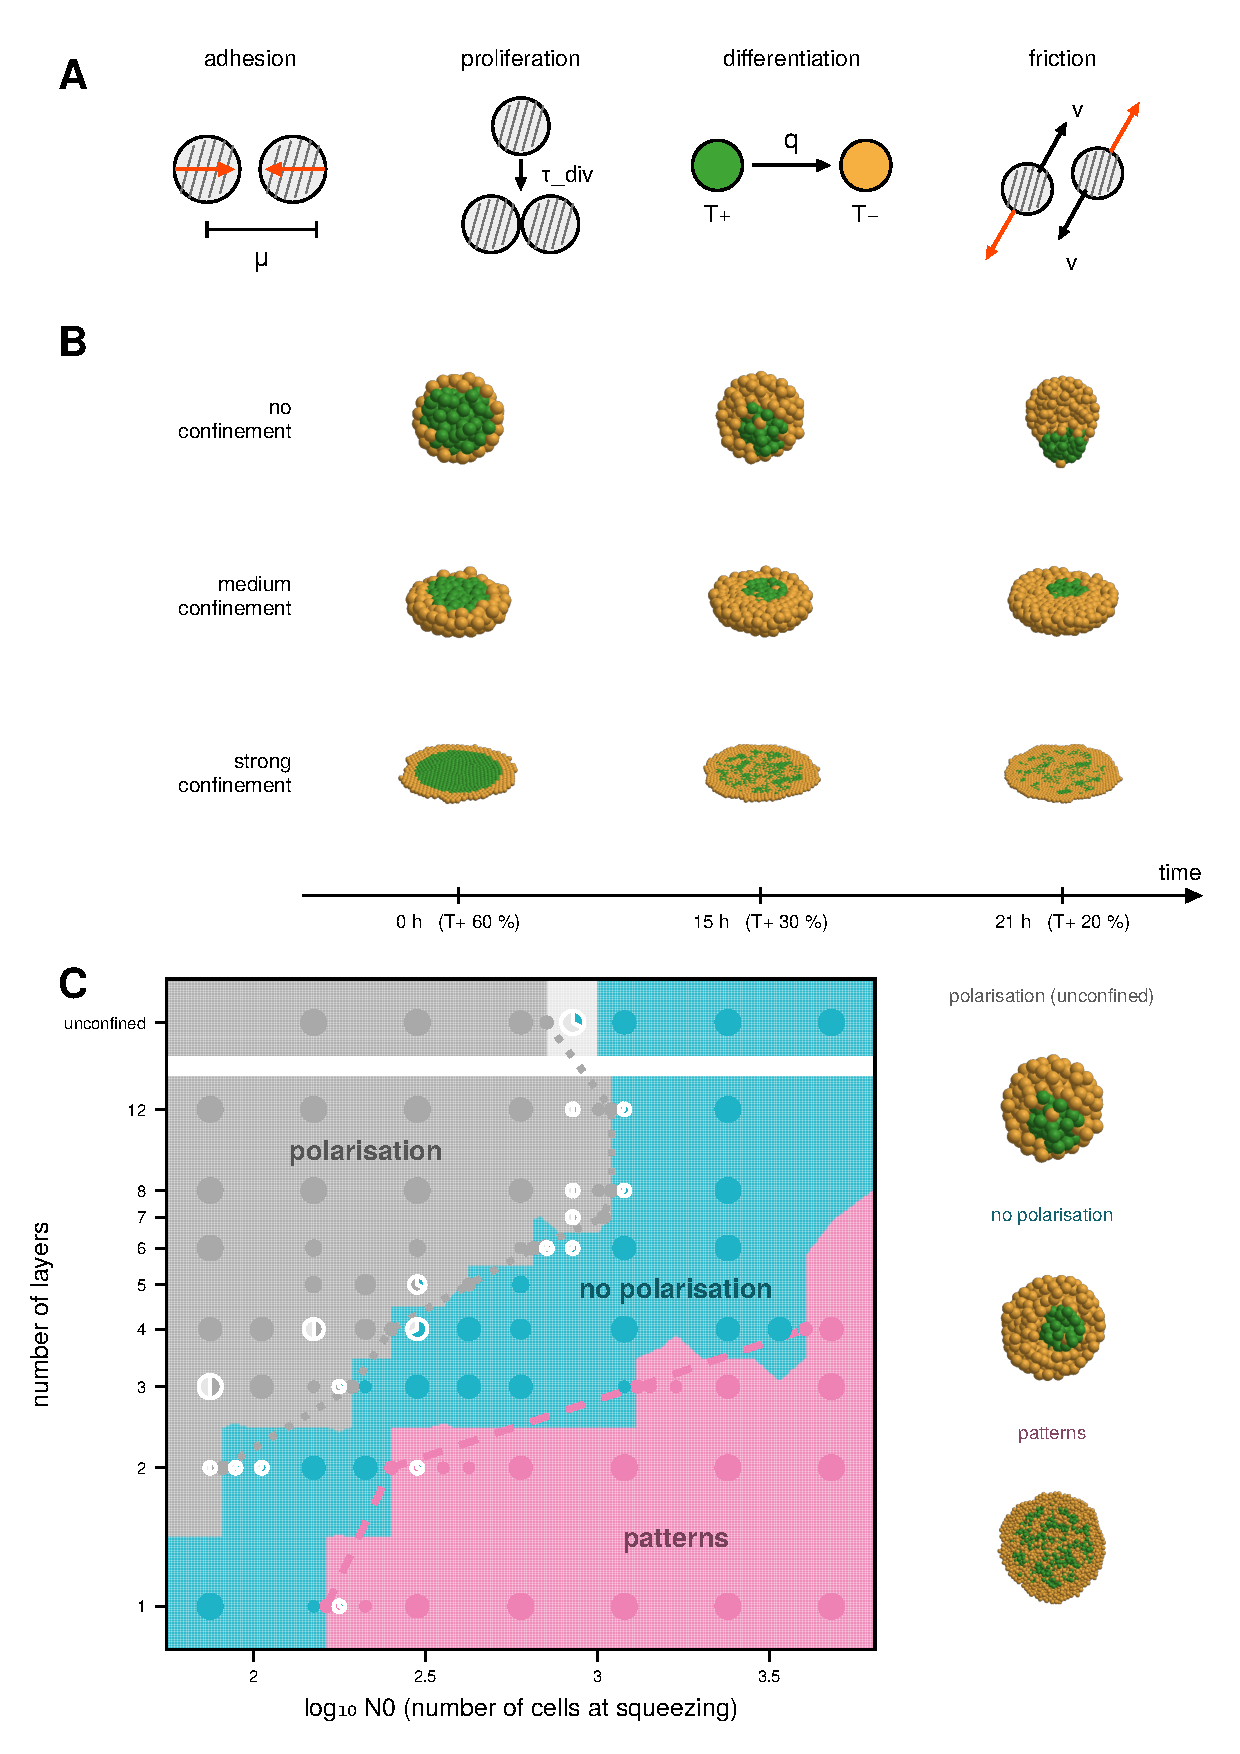
\includegraphics[width=0.85\linewidth]{figures/overview.pdf}
    \caption{Overview. (A) Model ingredients. (B) The same aggregate ($N_0=600$ cells) without confinement, with medium confinement (4 layers) and with strong confinement (1 layer), at the moment of squeezing and when $30\%$ and $20\%$ of the cells are still $T^+$. (C) Phase space: number of initial cells against the number of layers between the plates, with the unconfined aggregates on top.}
    \label{overview}
\end{figure}

\newpage
\section{The gastruloid physical model}

Since the July report the model has two cell states only, $B$ ($T^+$, T/Bra$^+$) and $C$ ($T^-$). The $A$ state, and with it the feedback on the transition rates, has been removed.

\begin{definition}
    The \textbf{equations of motion} are given by
    \begin{equation*}
        {\mathbf{v}}_i = \frac{1}{{\lambda} n_i} \sum_j {\mathbf{F}}_{ij} + \frac{\alpha}{n_i} \sum_j {\mathbf{v}}_j \,.
    \end{equation*}
    \textbf{Cellular forces} are given by
    \begin{equation*}
        \mathbf{F}_{ij}(s_i, s_j, d_{ij}) = f(d_{ij})\, \hat{\mathbf{r}}_{ij} \cdot
        \begin{cases}
            F_\text{rep}^{(s_i, s_j)}, & \text{if } d_{ij} \leq 2r \\
            F_\text{att}^{(s_i, s_j)}, & \text{if } 2r < d_{ij} < 2\mu r \\
            0, & \text{otherwise} \,,
        \end{cases}
    \end{equation*}
    where $s_i,s_j \in\{B,C\}$,
    ${d}_{ij} = {|\mathbf{x}_i - \mathbf{x}_j|}$,
    $\hat{\mathbf{r}}_{ij} = \frac{\mathbf{x}_i - \mathbf{x}_j}{|\mathbf{x}_i - \mathbf{x}_j|}$,
    and
    $$f(d_{ij}) = \left(\frac{2r}{d_{ij}} - 1\right)\left(\frac{2\mu r}{d_{ij}} - 1\right) \,.$$
\end{definition}

\begin{remark}
    In the code we set $\hat\alpha=\lambda\alpha$ and so
    \begin{equation*}
        {\mathbf{v}}_i = \frac{1}{{\lambda} n_i}\left( \sum_j {\mathbf{F}}_{ij} + \alpha \sum_j {\mathbf{v}}_j \right) \,.
    \end{equation*}
\end{remark}

\begin{remark}
    Pulling two attached cells apart costs the \textbf{adhesion energy}
    \begin{equation*}
        W_{XY} = \int_{2r}^{2\mu r} |F|\,\diff d = F_\text{att}^{(X,Y)}\, 2r\, A(\mu_{XY}) \,, \qquad A(\mu) = (1+\mu)\ln\mu - 2(\mu - 1) \,.
    \end{equation*}
    These energies set the surface tensions $\sigma_X = W_{XX}/2$ and the interfacial tension $\gamma_{BC} = (W_{BB} + W_{CC})/2 - W_{BC}$. Two aggregates glue without rounding into one sphere when $|\sigma_B - \sigma_C| < \gamma_{BC} < \sigma_B + \sigma_C$.
\end{remark}

\begin{definition}
    The \textbf{division time} is chosen uniformly at random from
    \begin{equation*}
        \text{U}\left(\tau_{div}(1-\sigma_{div}),\tau_{div}(1+\sigma_{div})\right) \,.
    \end{equation*}
\end{definition}

\begin{definition}
    The \textbf{transition rate} from $B$ to $C$ is constant,
    \begin{equation*}
        r_{B\rightarrow C} = q \,,
    \end{equation*}
    so every $B$ cell becomes $C$ with probability $q\,\Delta t$ per time step. There is no $A$ state and no feedback.
\end{definition}

\begin{definition}
    The \textbf{plates} sit at $z=0$ and $z=L$, with $L = 2.1\,r \times$ (number of layers). They are rigid: a cell touching a plate cannot move further into it, so the slab keeps its thickness during the whole simulation. A cell closer than $0.05$ to a plate also feels \textbf{plate friction}, an extra in-plane drag:
    \begin{equation*}
        v_{x,y} = \frac{F_{x,y} + \alpha \sum_j v_{j,(x,y)}}{\lambda n_i + \lambda_\text{wall}} \,.
    \end{equation*}
\end{definition}

\begin{definition}
    The \textbf{initial condition} is built in three steps:
    \begin{enumerate}
        \item One $C$ cell grows by division up to $N_0$ cells, between the plates if the aggregate is confined (the squeezing). The aggregate then relaxes for 100 time units.
        \item The innermost $60\%$ of the cells become $B$: a cylinder through the slab when confined, a sphere when unconfined. The time is reset to zero.
        \item After a short relaxation, $B$ cells differentiate to $C$ and all cells divide.
    \end{enumerate}
\end{definition}

\begin{remark}
    With $q = 0.004667$ the lifetime of a $B$ cell is $1/q \approx 214$ time units, about $14$ hours, so we read time with $1\,\text{h} \approx 15$ time units. The fraction of $B$ cells falls from $60\%$ to $20\%$ in about 21 hours, against 24 hours (from 72 to 96 h) in the experiments.
\end{remark}


\section{Description of the experiment}

First, we grow and differentiate a gastruloid aggregate before polarisation begins. Instead of the three-state description used in \cite{oriola} ($A\to B\to C$), we use two states. In this description, the resulting aggregate at this step is a spheroid with a central cluster of $T^+$ cells ($B$, about $60\%$ of the cells) and an outer layer of $T^-$ cells ($C$). If we were to let this further evolve, this cluster would move away from the center to the outer layer (polarisation).

Before this polarisation occurs, we confine this spherical aggregate between two plates. The result is a pancake-shaped aggregate inheriting the previous structure, which can then evolve in three ways:
\begin{enumerate}
    \item if the pancake is thin and its radius is small, the $B$ cluster remains in the center and all its cells eventually differentiate to $C$;
    \item if the pancake is thin and its radius is large enough, the cluster breaks into pattern-like structures, several loose $B$ islands spread across the whole aggregate;
    \item if the gap between the plates is large compared with the aggregate, it behaves as if it were not confined and polarises.
\end{enumerate}

The same number of cells that yields patterns for a given confinement thickness may not give rise to patterns for thicker \textit{pancakes}, since their radius will be smaller.


\section{Simulations}

The main challenge of the simulations is to obtain the three behaviours above for several confinement thicknesses and, with the same parameters, to replicate the following phenomena observed in nonconfined gastruloid aggregates:
\begin{enumerate}
    \item Polarisation of the central cluster.
    \item Fusion: two $B$ aggregates or two $C$ aggregates fuse into one, whereas a $B$ and a $C$ aggregate stay glued together without rounding into one sphere.
\end{enumerate}

All the parameters, and how they changed since the July report, are in Table~\ref{parameters}. All the figures are three-dimensional; a top view leaves out the cells above the mid-plane, since the outer $C$ cells would hide the $B$ pattern otherwise.

\subsection{Initial condition}

Figure~\ref{initial-condition} shows the seeded aggregate. We also tried a diluted core (a quarter of the $B$ cells outside the core), but it makes small squeezed aggregates polarise, so the sharp core is used.

\begin{figure}[htbp]
    \centering
    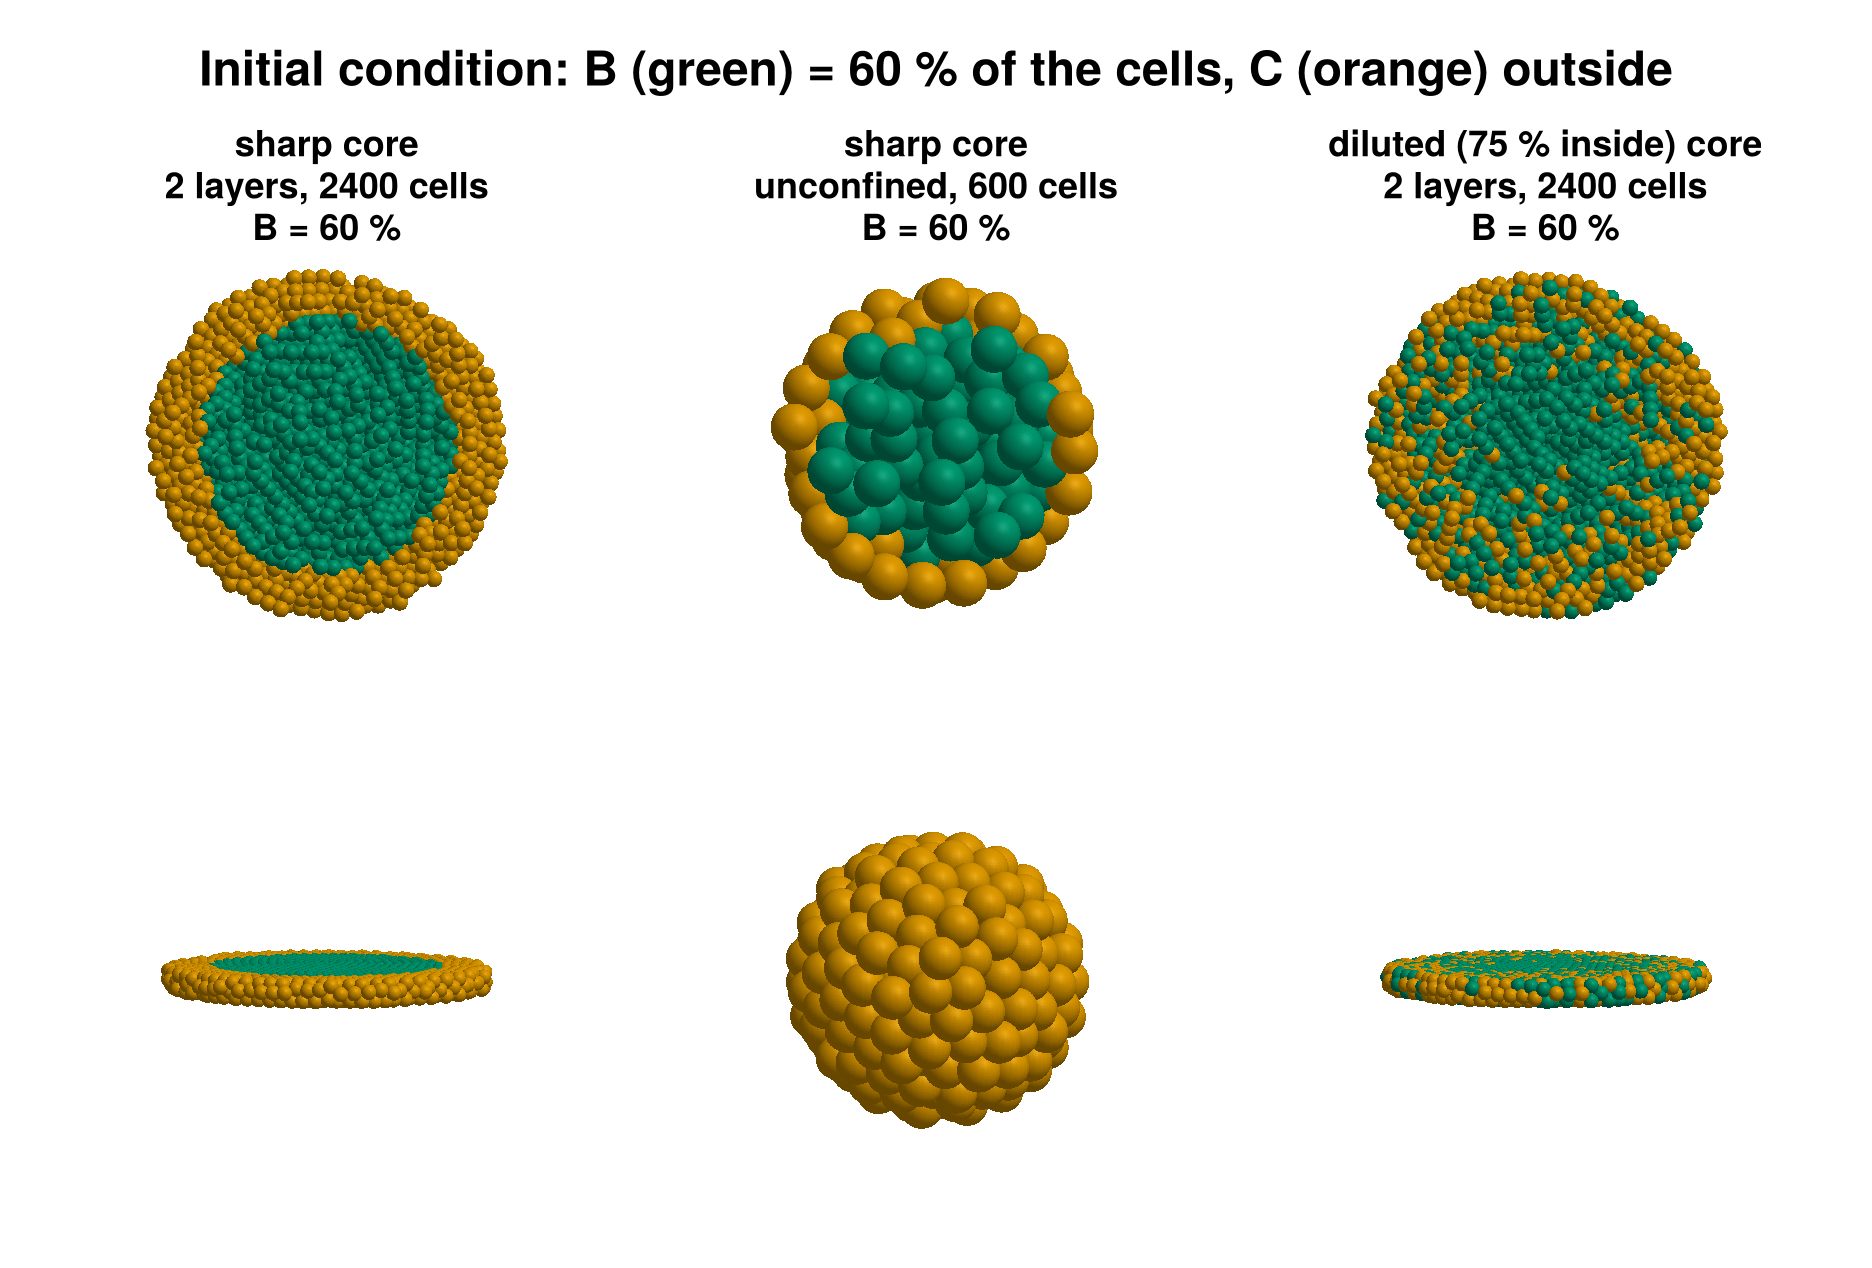
\includegraphics[width=0.8\linewidth]{figures/fig1_initial_condition.png}
    \caption{Initial condition: $60\%$ of the cells are $B$ (green), the innermost ones. Left: 2 layers, $N_0=2400$. Middle: unconfined, $N_0=600$. Right: a diluted core, which is not used.}
    \label{initial-condition}
\end{figure}

\subsection{Fusion}

Two aggregates of 150 cells of a single type are placed in contact and followed for 24 hours without division or differentiation (Figure~\ref{fusion}). The distance between their centres over the sum of their radii of gyration is about $1.6$ when they just touch and $0.5$ for a single sphere. $BB$ and $CC$ fuse ($0.54$ and $0.56$), whereas $BC$ glues and keeps two lobes ($0.91$, close to the $0.95$ of Sotiris' reference).

\begin{figure}[htbp]
    \centering
    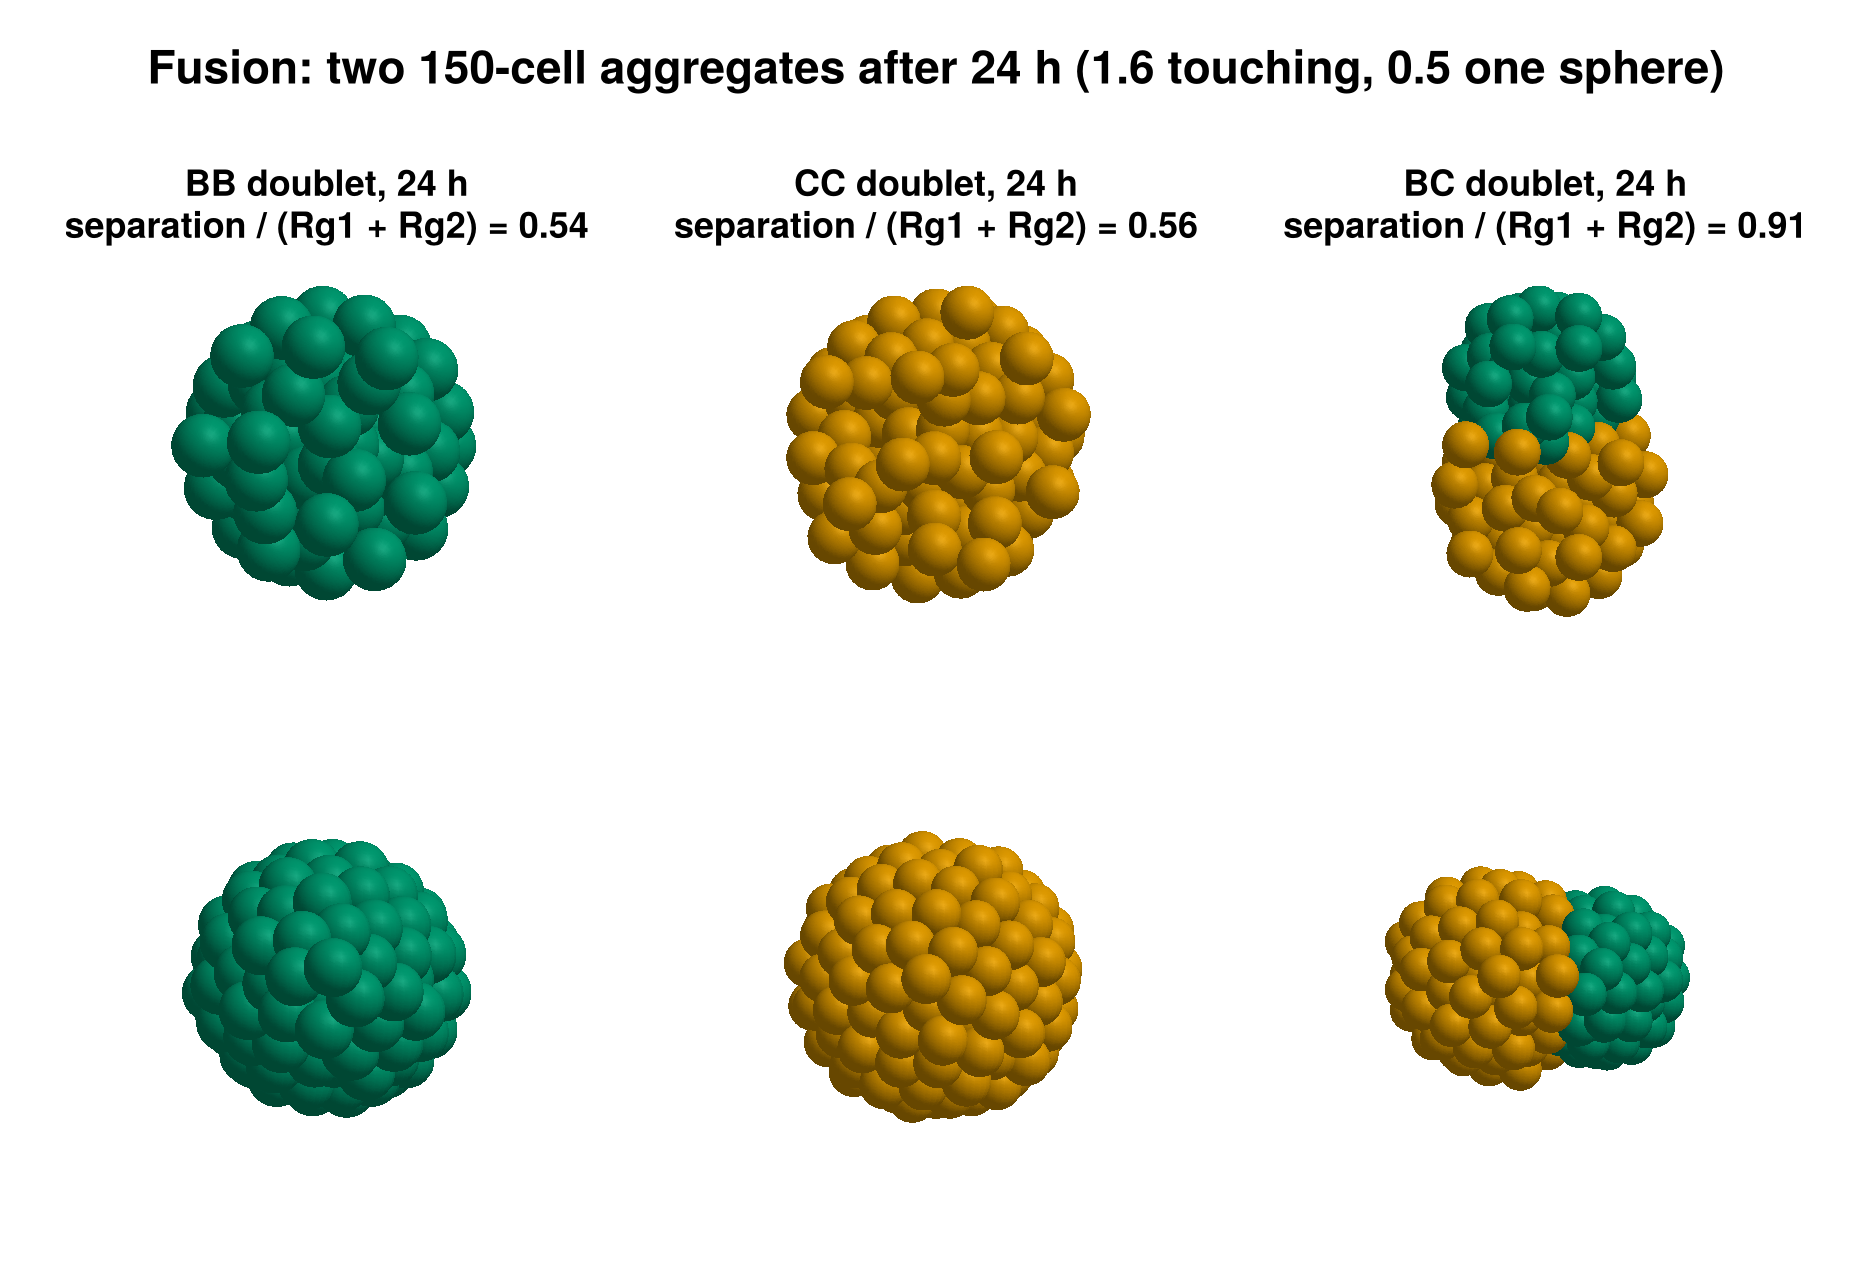
\includegraphics[width=0.75\linewidth]{figures/fig5_fusion.png}
    \caption{Fusion assay after 24 hours: $BB$, $CC$ and $BC$ doublets.}
    \label{fusion}
\end{figure}

\subsection{Polarisation}

Unconfined aggregates of up to $N_0 = 600$ cells polarise before $B$ runs out (Figure~\ref{polarisation}). Larger aggregates ($N_0 = 1200$ to $4800$) still have a central cluster when $20\%$ of the cells are $B$, and the largest never polarise.

\begin{figure}[htbp]
    \centering
    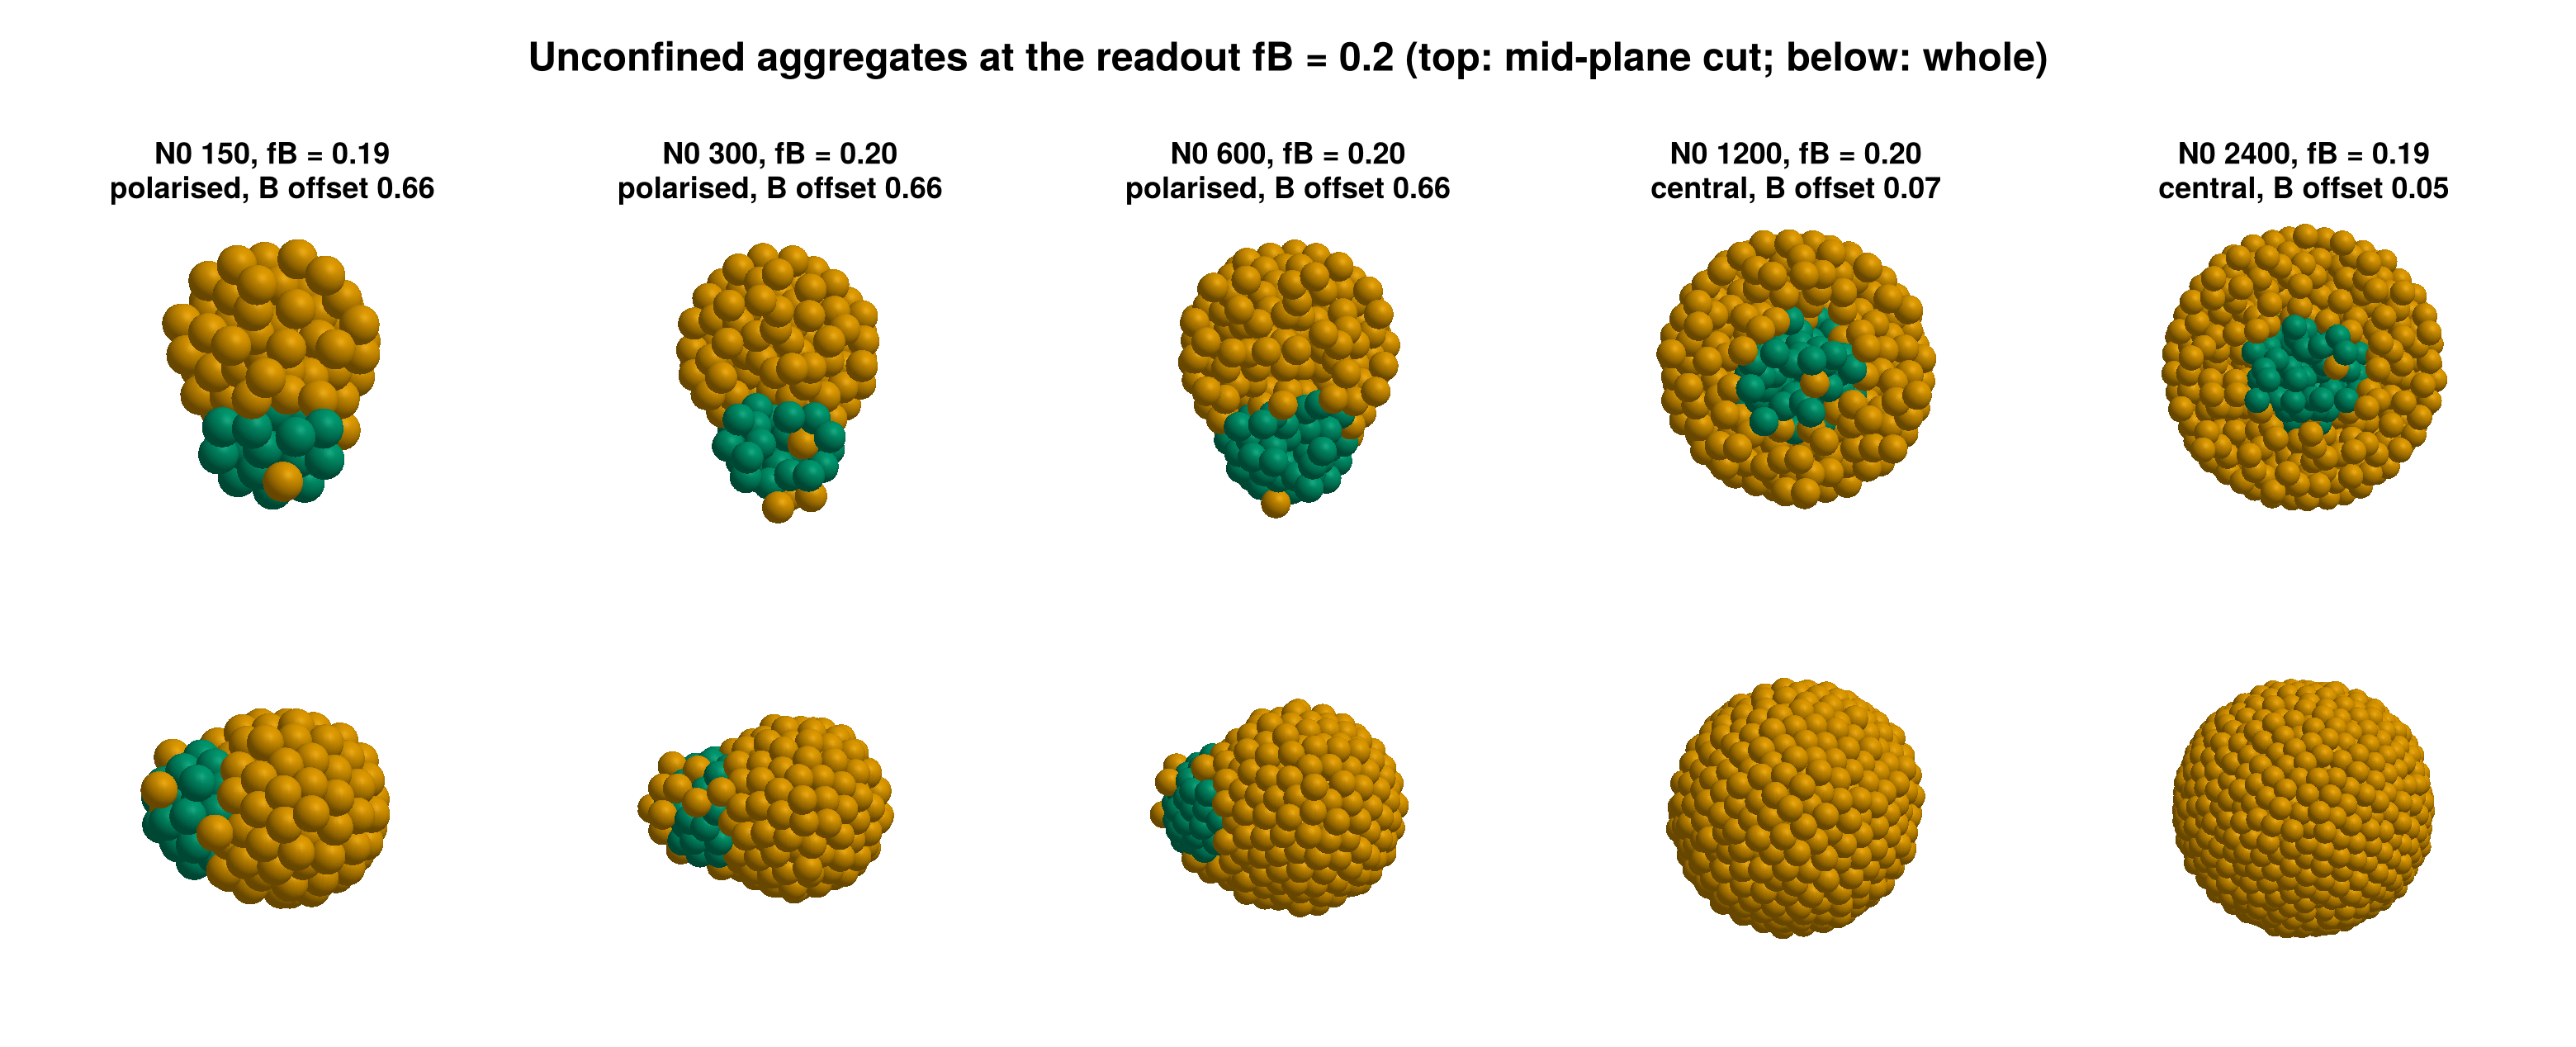
\includegraphics[width=\linewidth]{figures/fig4_unconfined.png}
    \caption{Unconfined aggregates of $N_0 = 150$ to $2400$ cells when $20\%$ of the cells are $B$. Top: cut at the mid-plane; bottom: whole aggregate. Rotated so that $B$ points to the right.}
    \label{polarisation}
\end{figure}

\subsection{Confinement}

Figure~\ref{behaviours} follows the same aggregate under no, medium and strong confinement. Figure~\ref{patterns} shows patterns from one to four layers.

\begin{figure}[htbp]
    \centering
    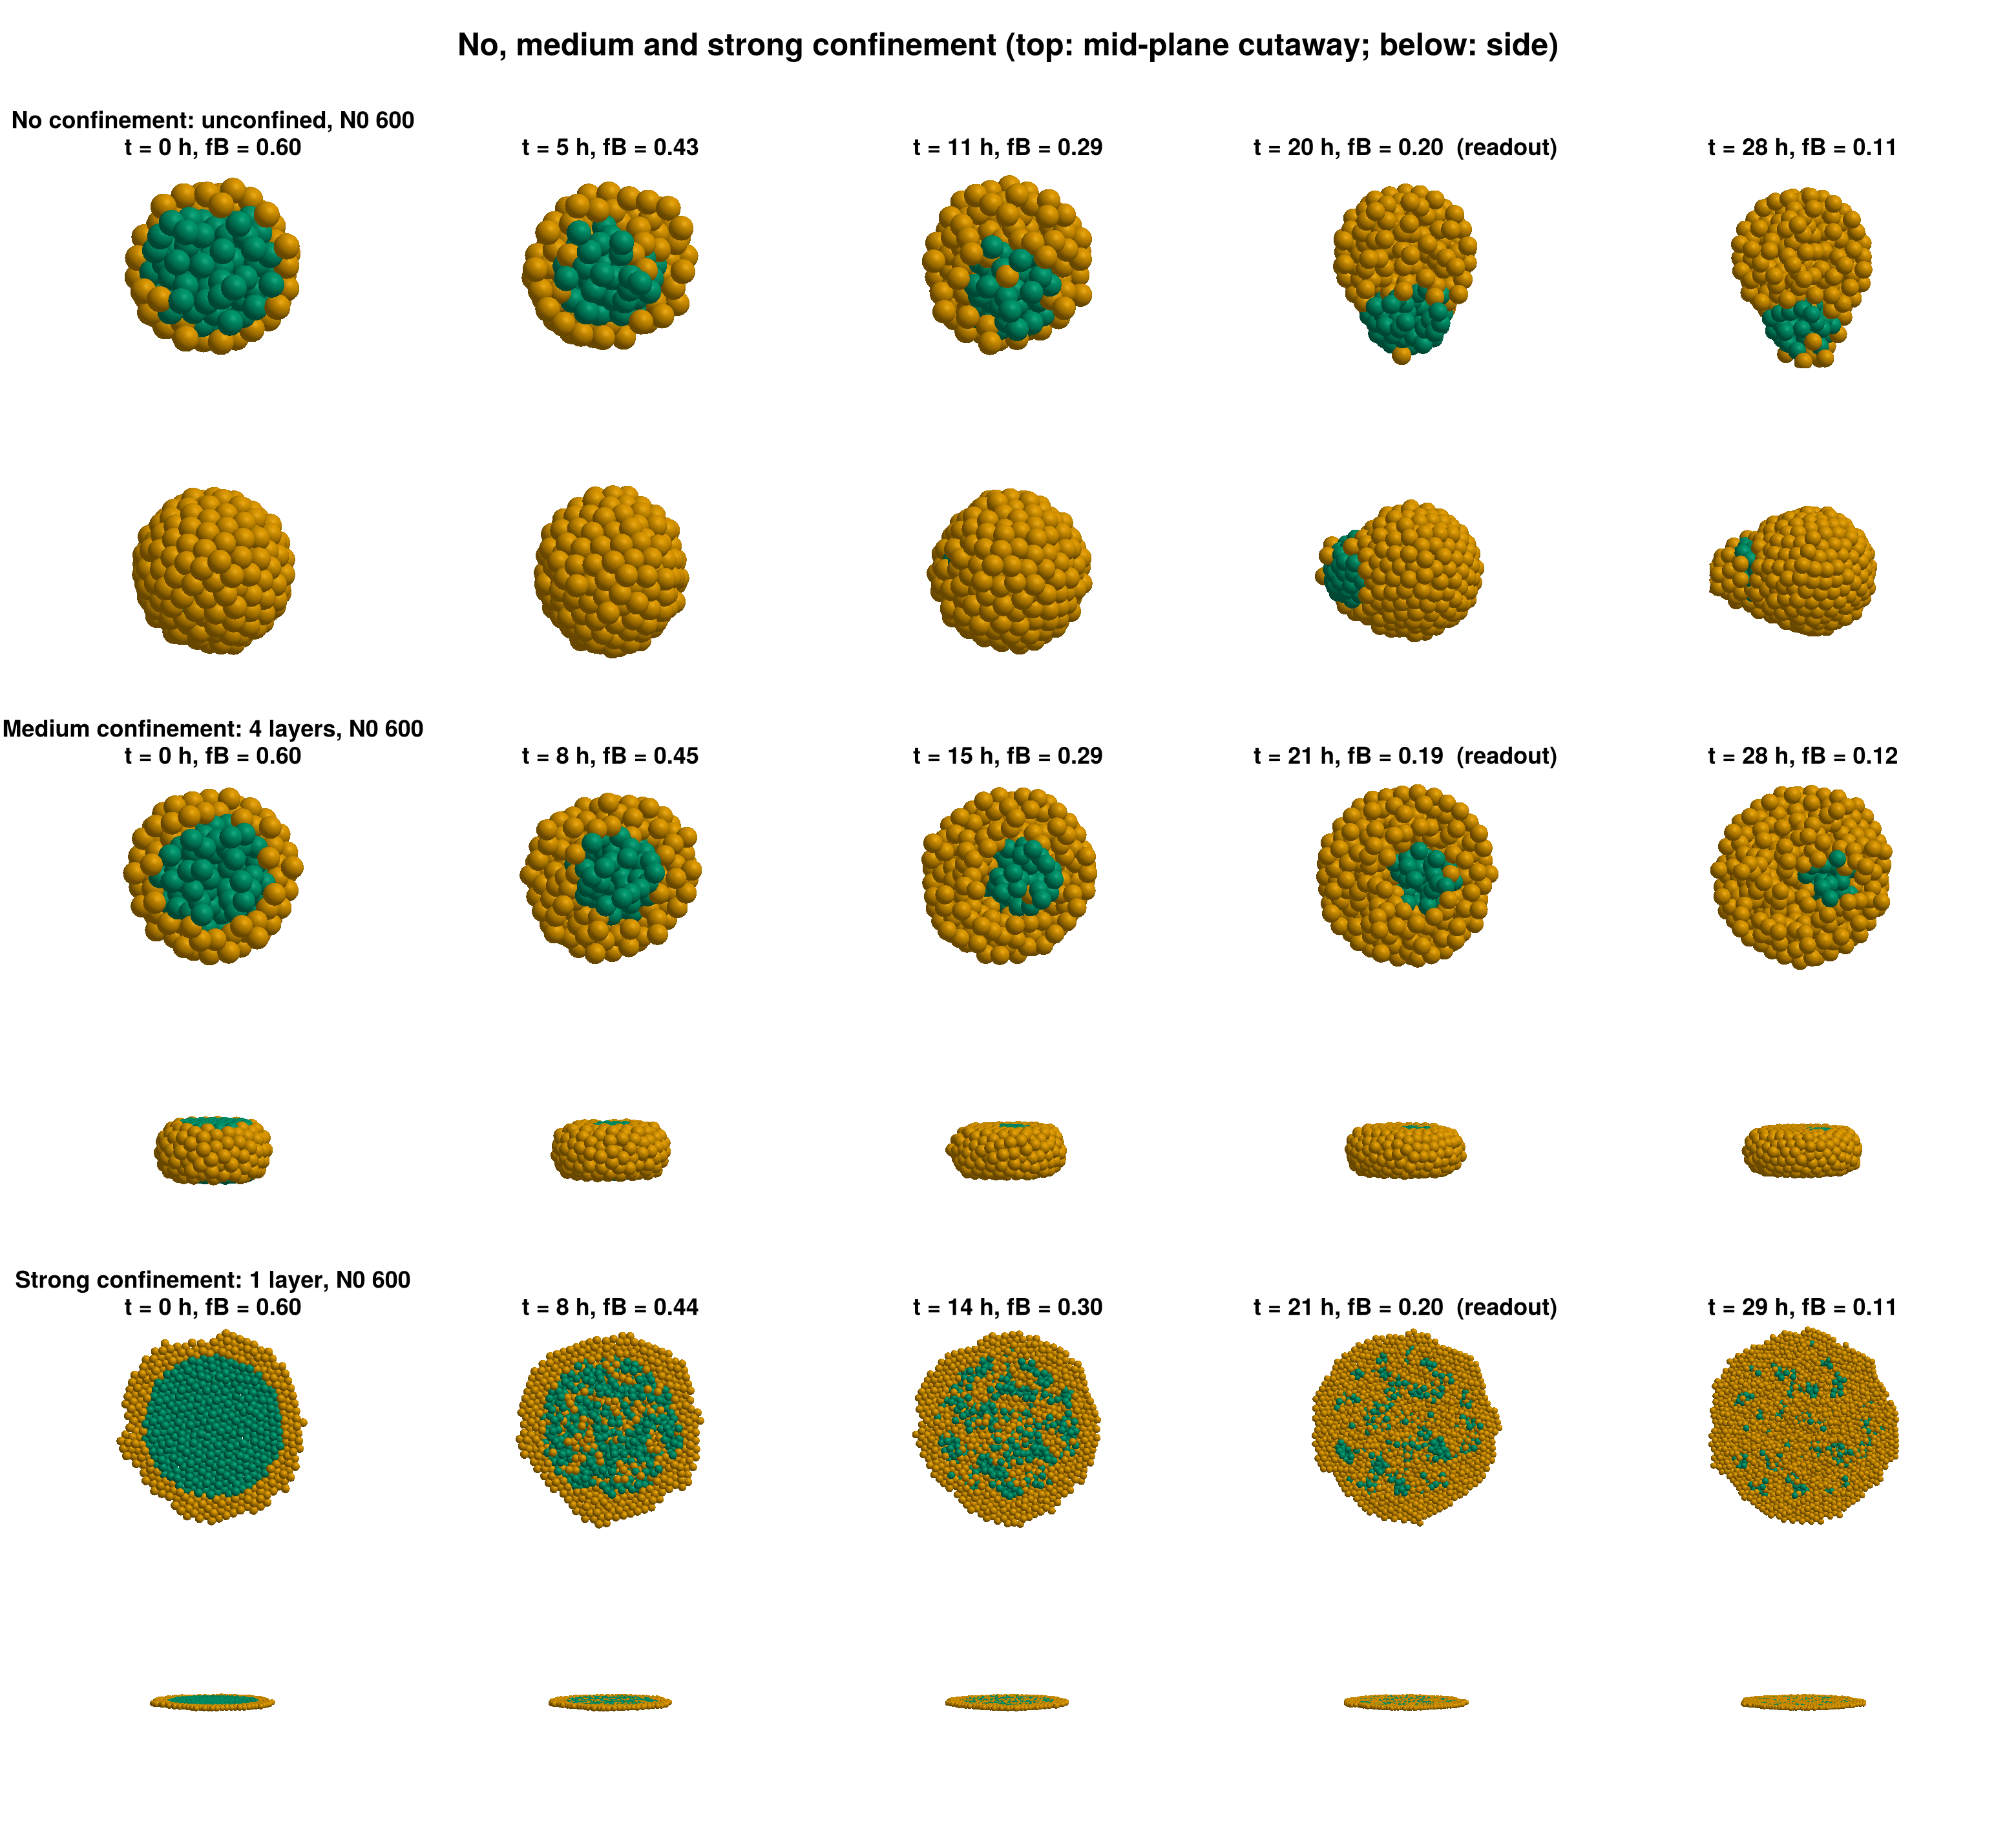
\includegraphics[width=\linewidth]{figures/fig2_behaviours.png}
    \caption{$N_0=600$ cells with no confinement (polarises), 4 layers (central cluster that differentiates away) and 1 layer (islands), from the seeding to $12\%$ of $B$ cells. The readout is at $20\%$.}
    \label{behaviours}
\end{figure}

\begin{figure}[htbp]
    \centering
    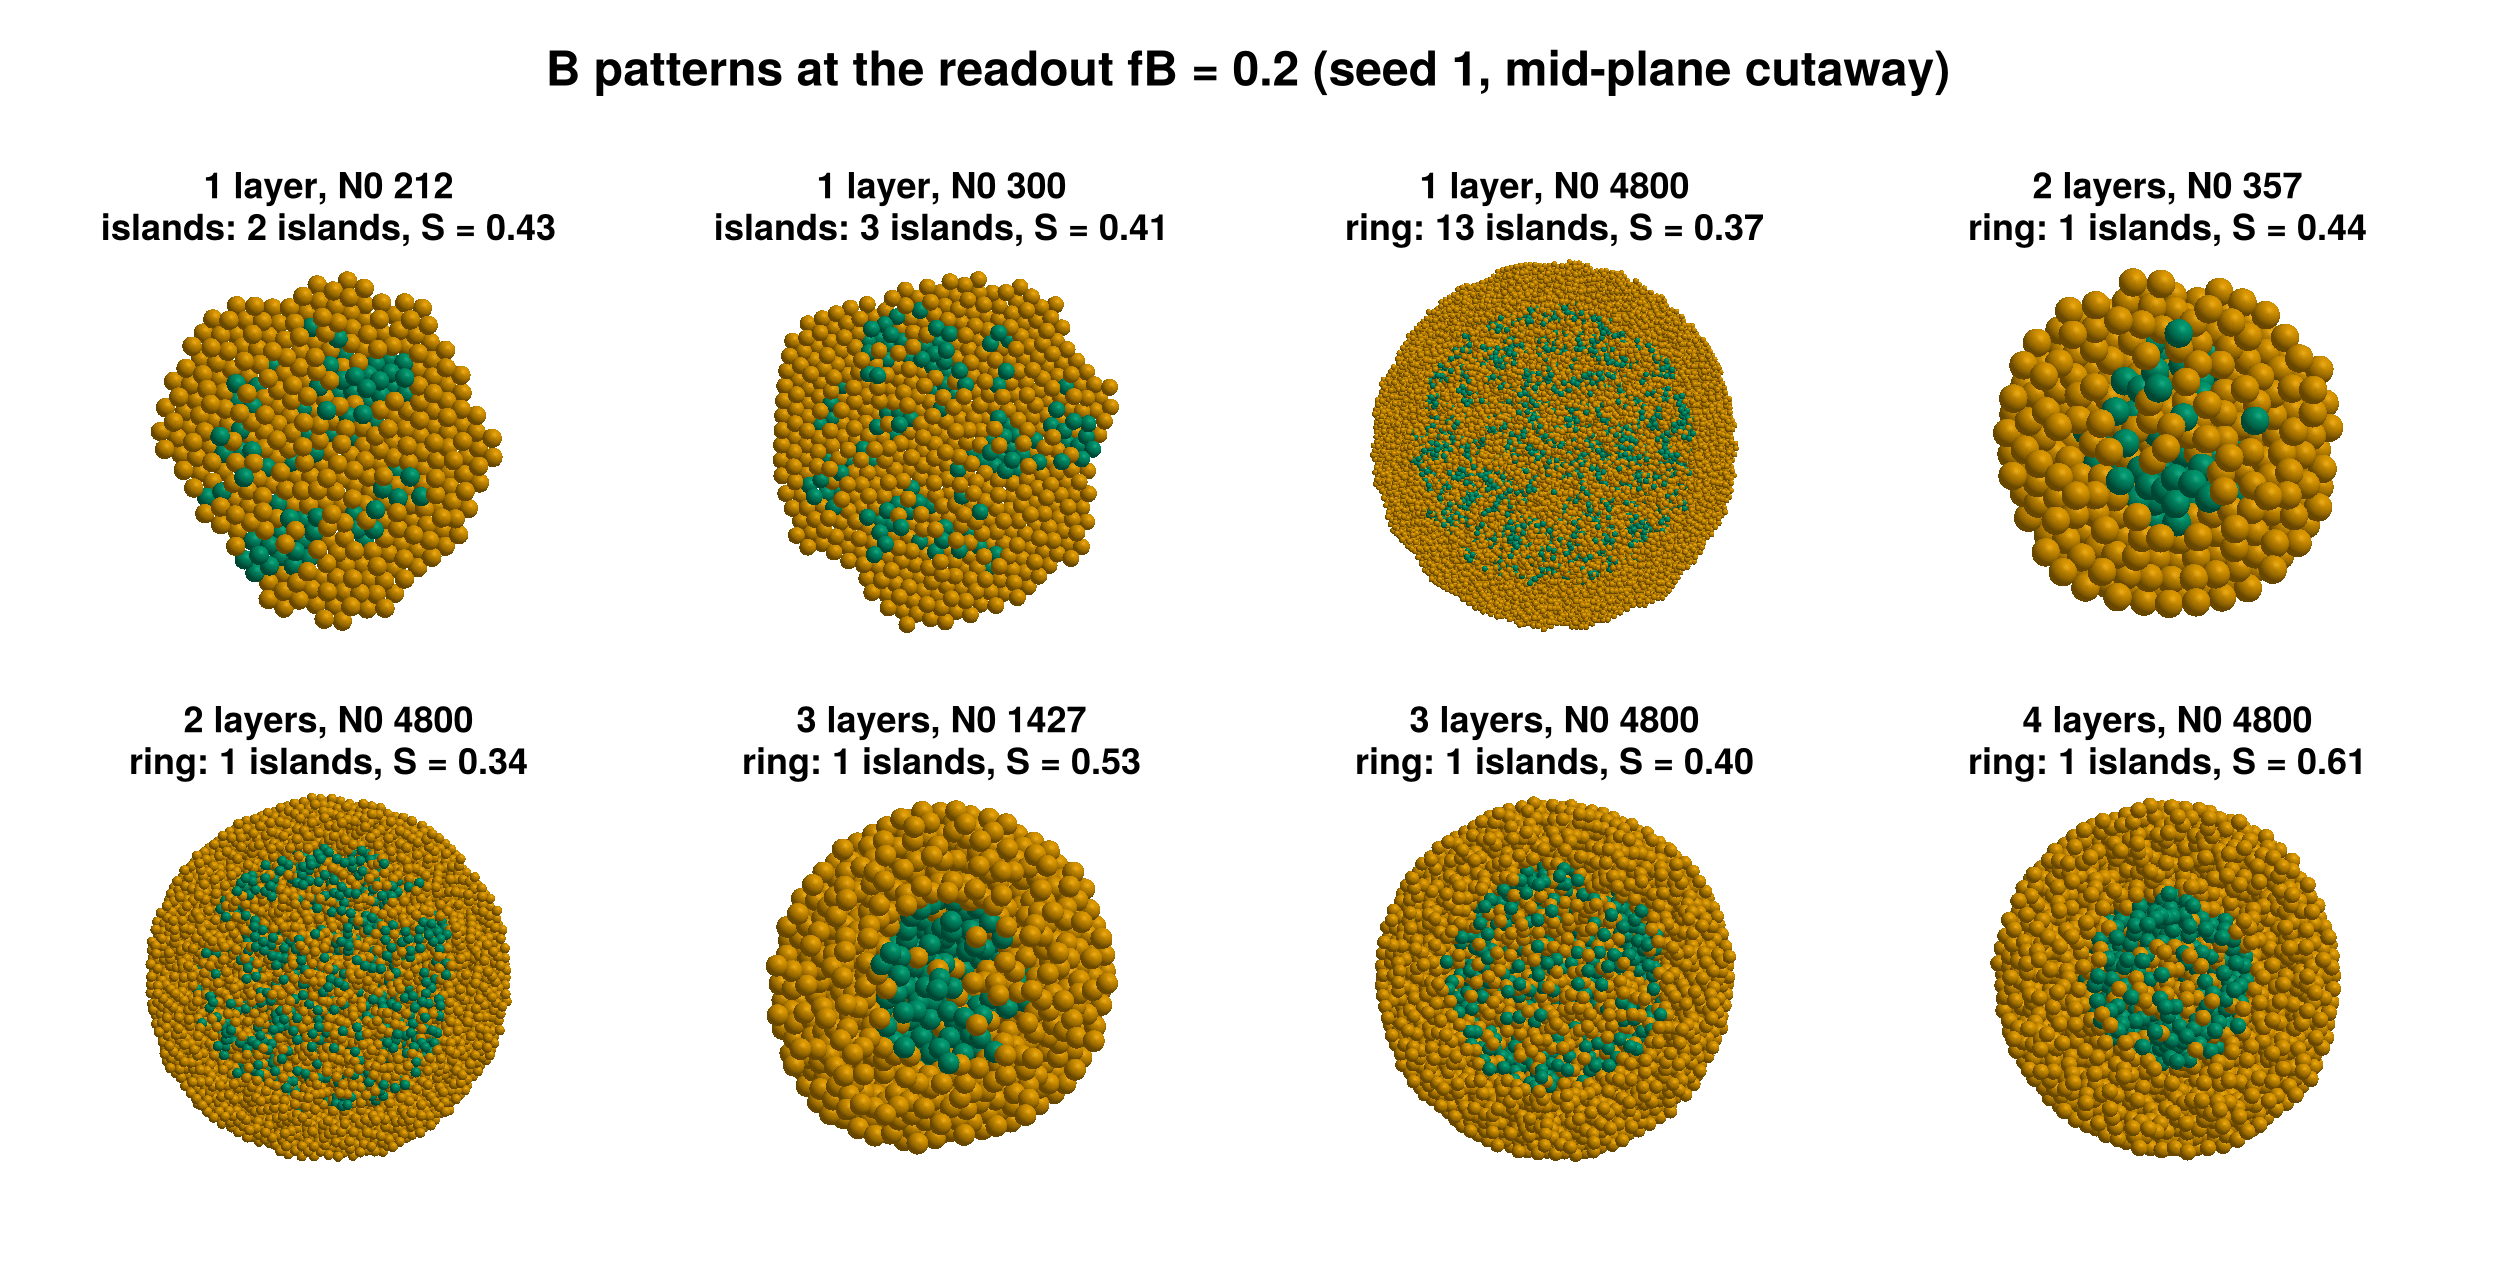
\includegraphics[width=\linewidth]{figures/fig3_patterns.png}
    \caption{Patterns when $20\%$ of the cells are $B$, from one to four layers.}
    \label{patterns}
\end{figure}

In thick slabs the pattern starts as a ring: the core hollows out and then breaks into islands (Figure~\ref{ring}).

\begin{figure}[htbp]
    \centering
    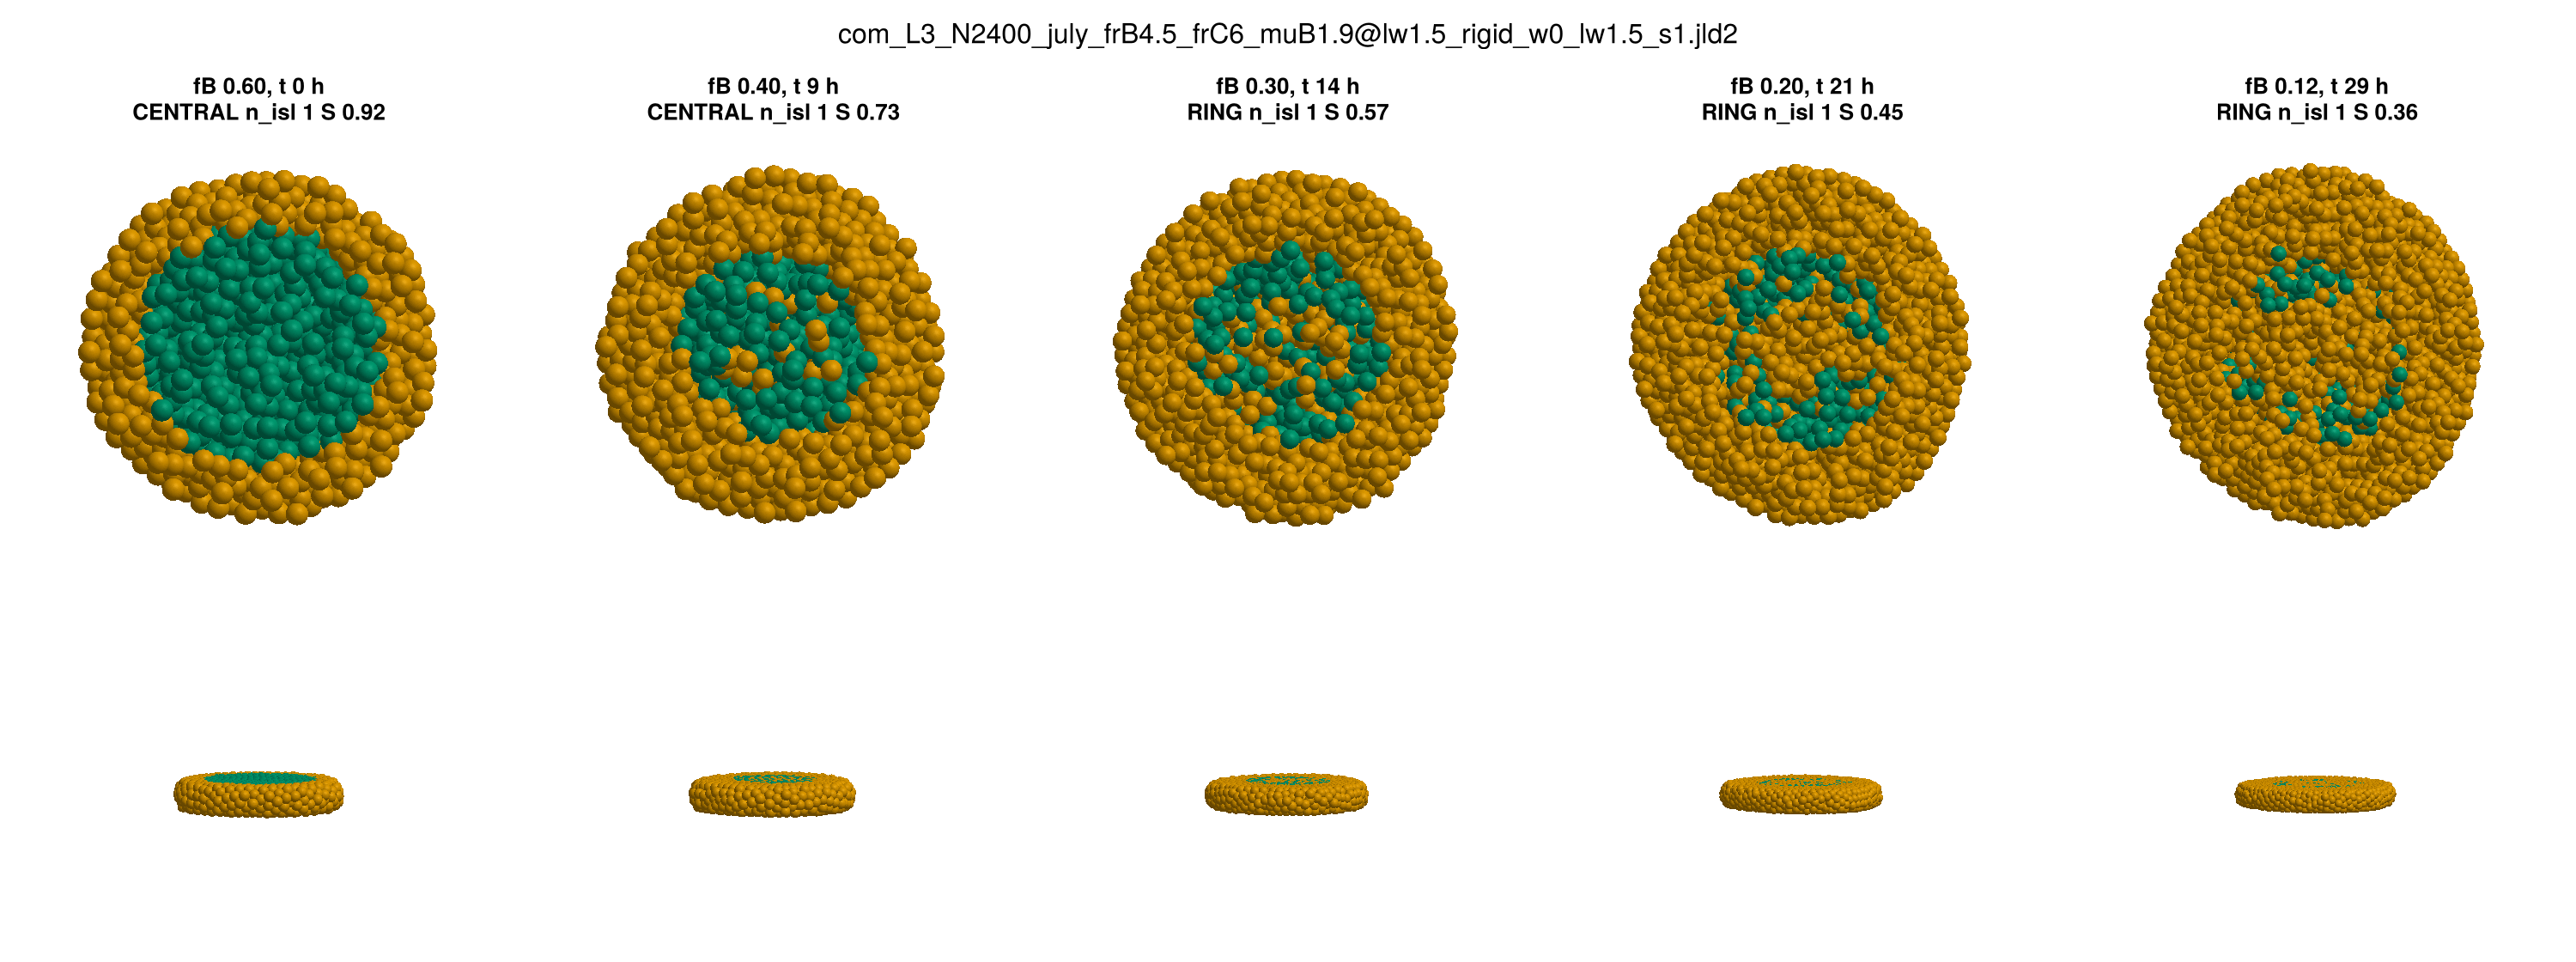
\includegraphics[width=\linewidth]{figures/ring-3layers.png}
    \caption{Three layers, $N_0 = 2400$: the central cluster hollows into a ring, which breaks into islands. Top: cut at the mid-plane; bottom: side view.}
    \label{ring}
\end{figure}

\subsection{Patterns in thick slabs}

With the parameters of early October, every slab of three or more layers ended as one compact central cluster, at any $N_0$ up to 4800. Table~\ref{attempts} lists what we tried at three layers and $N_0 = 2400$. The salt-and-pepper start is the one the July runs used: $75\%$ $B$, $15\%$ $A$ and $10\%$ $C$, shuffled inside the core.

\begin{table}[htbp]
    \centering
    {\small
    \begin{tabular}{lll}
        \hline
        \textbf{Change} & \textbf{Outcome} & \textbf{Looseness $S$} \\
        \hline
        $B$ fraction $65\%$ instead of $60\%$ & central & 0.88 \\
        $B$ cells scattered outside the core ($10$ to $30\%$ of them) & central & 0.86--0.89 \\
        $C$ cells mixed into the core ($10$ to $30\%$ of it, as in July) & central & 0.89--0.91 \\
        Spring plates (July) instead of rigid ones & central & 0.91 \\
        Plate friction 5 instead of 1.5 & central & 0.89 \\
        July mechanics ($F_\text{rep}^{BB}=3$, $F_\text{rep}^{CC}=5.1$) & central & 0.90--0.93 \\
        $F_\text{att}^{CC}$: $3 \to 3.6$ & central & 0.88 \\
        $F_\text{att}^{BB}$: $6.4 \to 5.6$ & central, looser & 0.72 \\
        $\lambda$ multiplied by 2, 3 or 4 & central (and no polarisation) & 0.52--0.84 \\
        $\mu_{BB}$: $2 \to 1.85$ or $1.8$ & $B$ dissolves into $C$ & 0.30--0.35 \\
        $\boldsymbol{\mu_{BB}}\colon \mathbf{2 \to 1.9}$ & \textbf{ring, then islands} & \textbf{0.45} \\
        \hline
    \end{tabular}
    }
    \caption{What we tried to obtain patterns at three layers ($N_0 = 2400$). $S$ is about $0.9$ for a compact cluster and $0.4$--$0.6$ for loose patterns.}
    \label{attempts}
\end{table}

What changes the outcome is the cohesion of the $B$ tissue. In a slab of one or two layers, the $C$ cells that appear inside the $B$ core cannot get out, since cells cannot pass each other, and they split the core. From three layers on, cells pass over and under each other, and a cohesive $B$ core squeezes the new $C$ cells out and stays as one cluster. Shortening the $B$--$B$ attraction range from $\mu_{BB}=2$ to $1.9$ lowers the $B$--$B$ adhesion energy from $W_{BB}=1.02$ to $0.79$, still above $W_{CC}=0.65$. Then small cores stay compact, but a large core in a thick slab opens into a ring. It is the energy and not the range: with $\mu_{BB} = 1.8$ and $F_\text{att}^{BB}$ raised to keep $W_{BB} = 1.02$, the core stays compact. At $\mu_{BB} = 1.85$ ($W_{BB} \approx W_{CC}$), $B$ is no longer more cohesive than $C$ and simply dissolves into it, even in small aggregates (Figure~\ref{dissolves}).

\begin{figure}[htbp]
    \centering
    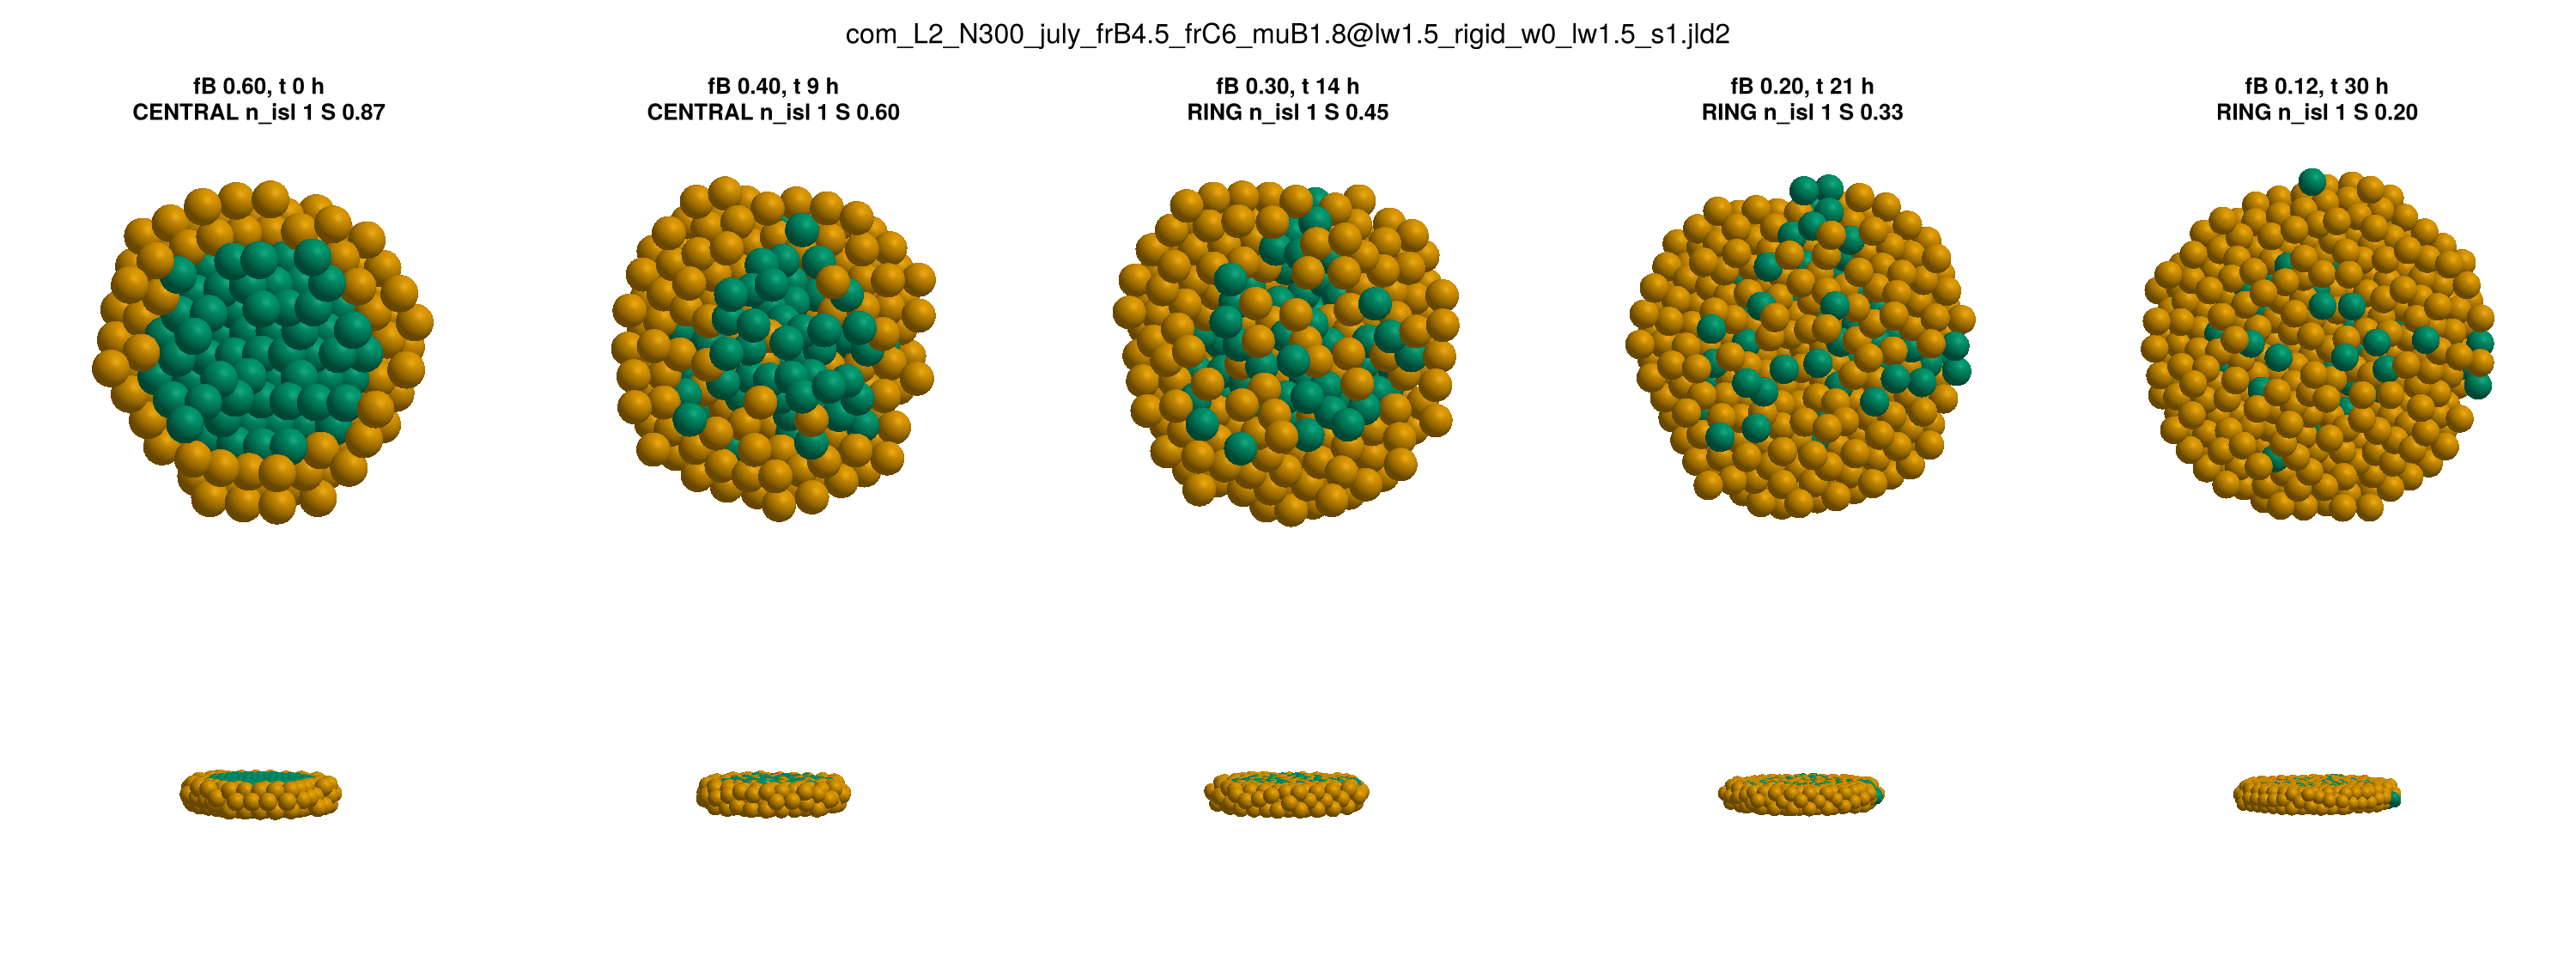
\includegraphics[width=\linewidth]{figures/dissolves-muBB1.8.png}
    \caption{With $\mu_{BB}=1.8$ the $B$ cells dissolve into the $C$ tissue (2 layers, $N_0 = 300$).}
    \label{dissolves}
\end{figure}

The new parameter set keeps the other behaviours: small squeezed aggregates keep a central cluster, monolayers give sparse islands, unconfined aggregates polarise, and $BC$ fusion glues.

\subsection{Phase space}

Finally, we compute the phase space relating the outcome, the number of layers and the number of cells $N_0$ at the moment of squeezing (Figure~\ref{phase-space}), with 2 or 3 simulations per point (178 in total). The outcome is read when $20\%$ of the cells are $B$ (96 h in the experiments) and classified as central cluster, pattern (a ring or islands), polarised, or other.

\begin{figure}[htbp]
    \centering
    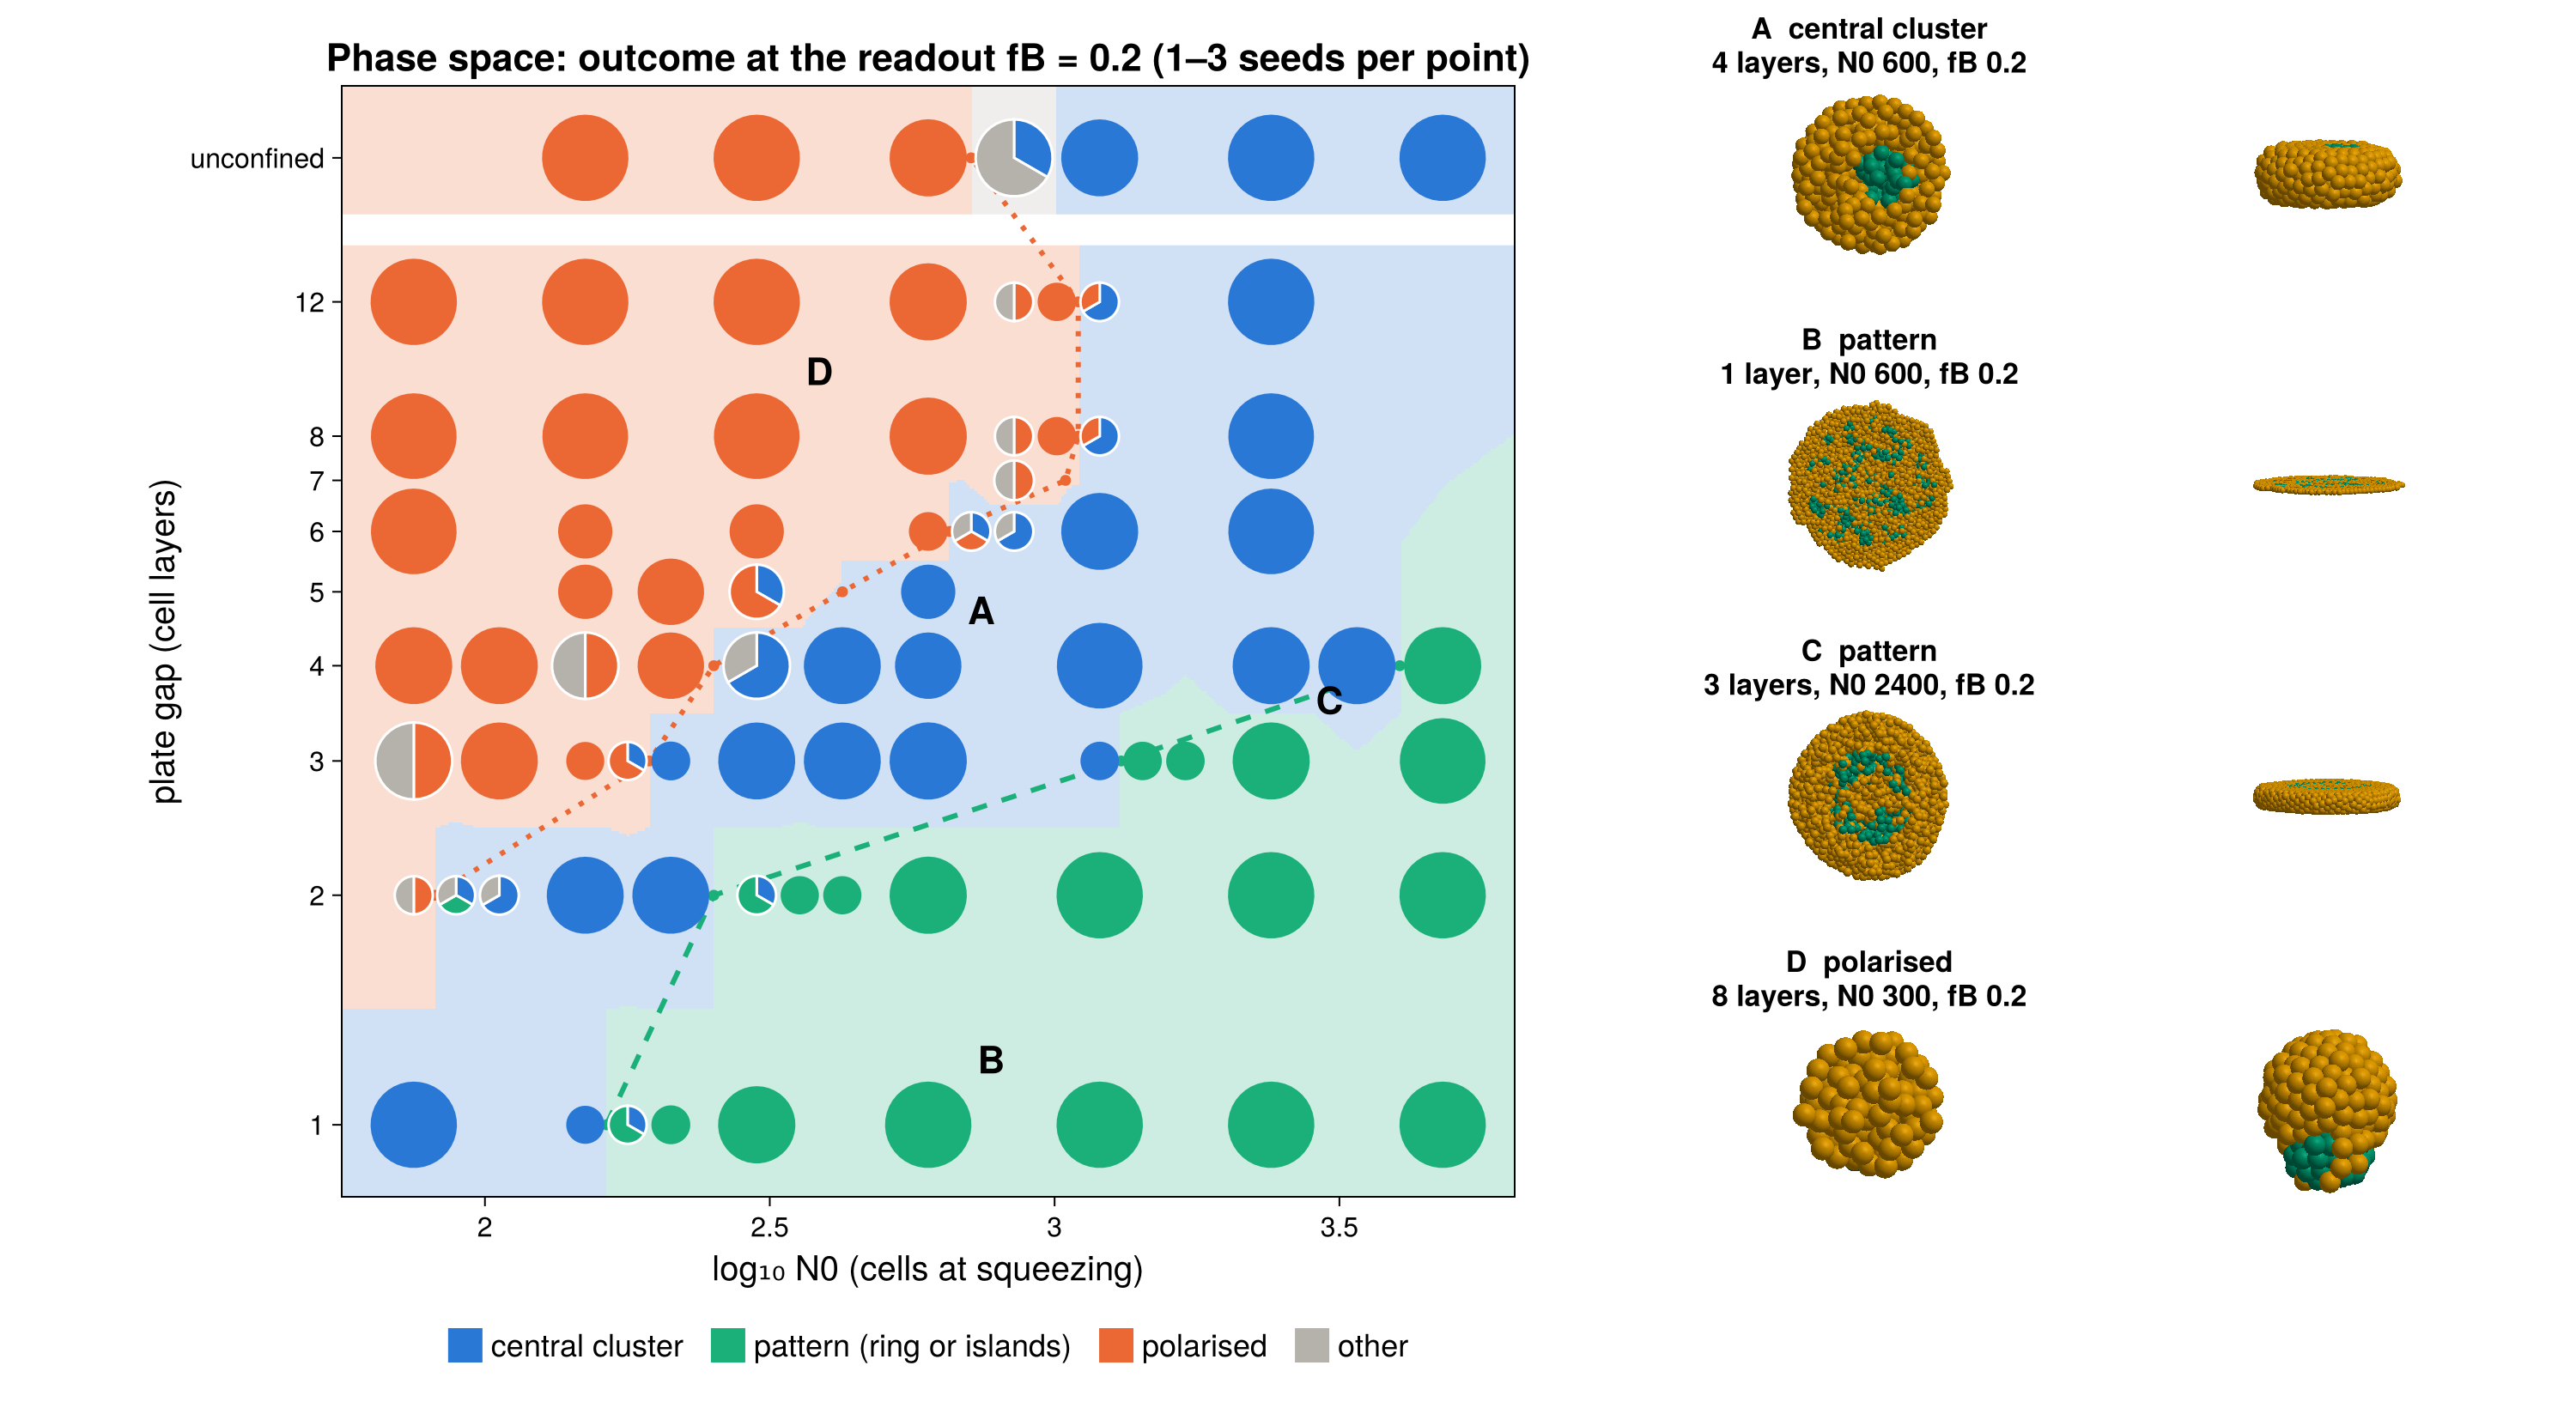
\includegraphics[width=\linewidth]{figures/phase_space.png}
    \caption{Phase space. Each point is a pie of the outcomes of its simulations; the background is the outcome of the nearest point. Dashed: patterns from here on; dotted: polarised up to here. Right: examples of each outcome.}
    \label{phase-space}
\end{figure}

\begin{table}[htbp]
    \centering
    {\small
    \begin{tabular}{cccc}
        \hline
        \textbf{Layers} & \textbf{Polarised up to $N_0$} & \textbf{Central cluster} & \textbf{Patterns from $N_0$} \\
        \hline
        1 & -- & 75--150 & $\approx 160$ \\
        2 & 75 & 89--212 & $\approx 250$ \\
        3 & 150--178 & 212--1200 & $\approx 1300$ \\
        4 & 212 & 300--3394 & between 3394 and 4800 \\
        6--12 & 600--1000 & up to 2400 & none up to 2400 \\
        unconfined & 600 & 849--4800 & none up to 4800 \\
        \hline
    \end{tabular}
    }
    \caption{The thresholds of Figure~\ref{phase-space}.}
    \label{thresholds}
\end{table}

The threshold for patterns grows quickly with the thickness, from $N_0 \approx 160$ cells at one layer to about 4000 at four layers. Plotted against the diameter of the pancake at the moment of squeezing (Figure~\ref{phase-space-diameter}), the threshold varies much less: patterns appear once the pancake is about 8 to 17 cell diameters wide (roughly 80 to 170~$\mu$m). Most of the effect of the thickness is therefore that a thicker slab needs many more cells to reach the same width.

\begin{figure}[htbp]
    \centering
    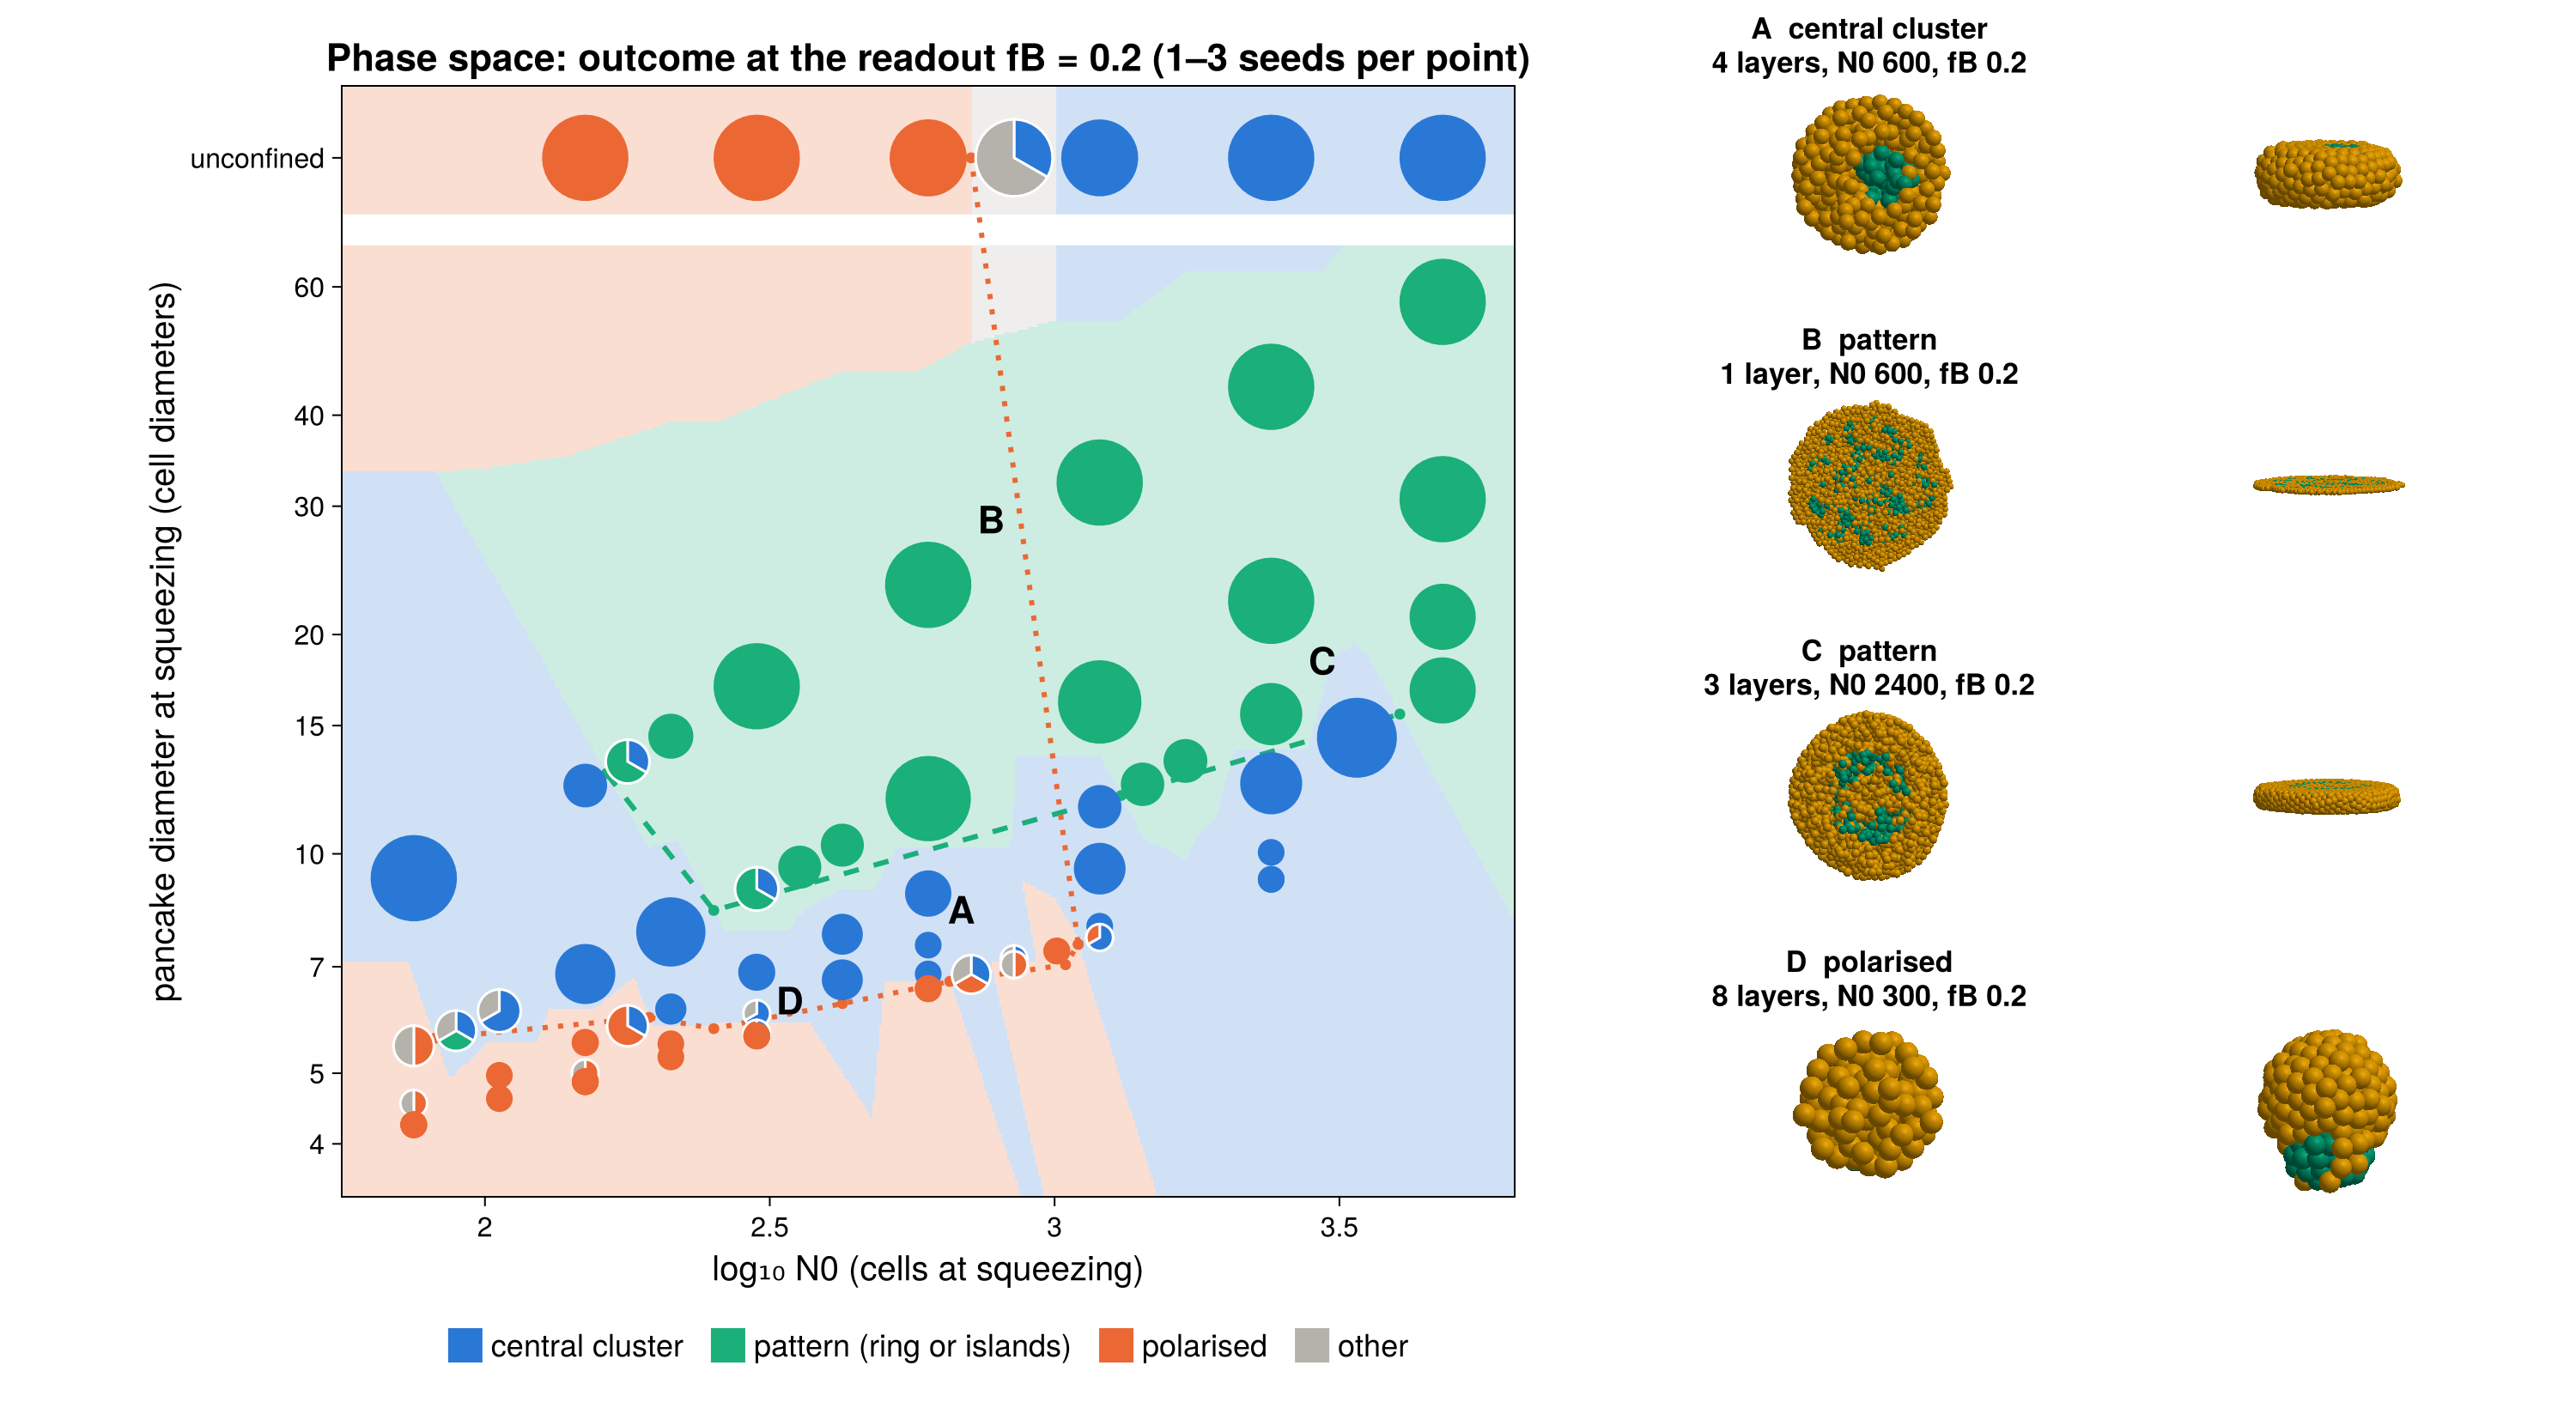
\includegraphics[width=\linewidth]{figures/phase_space_diameter.png}
    \caption{The same phase space against the diameter of the pancake at the moment of squeezing, in cell diameters.}
    \label{phase-space-diameter}
\end{figure}

The outcome depends on when it is read. Figure~\ref{phase-space-late} shows the same simulations when only $12\%$ of the cells are $B$: the rings break into islands, larger aggregates polarise late, and the smallest monolayer patterns shrink back to a central cluster.

\begin{figure}[htbp]
    \centering
    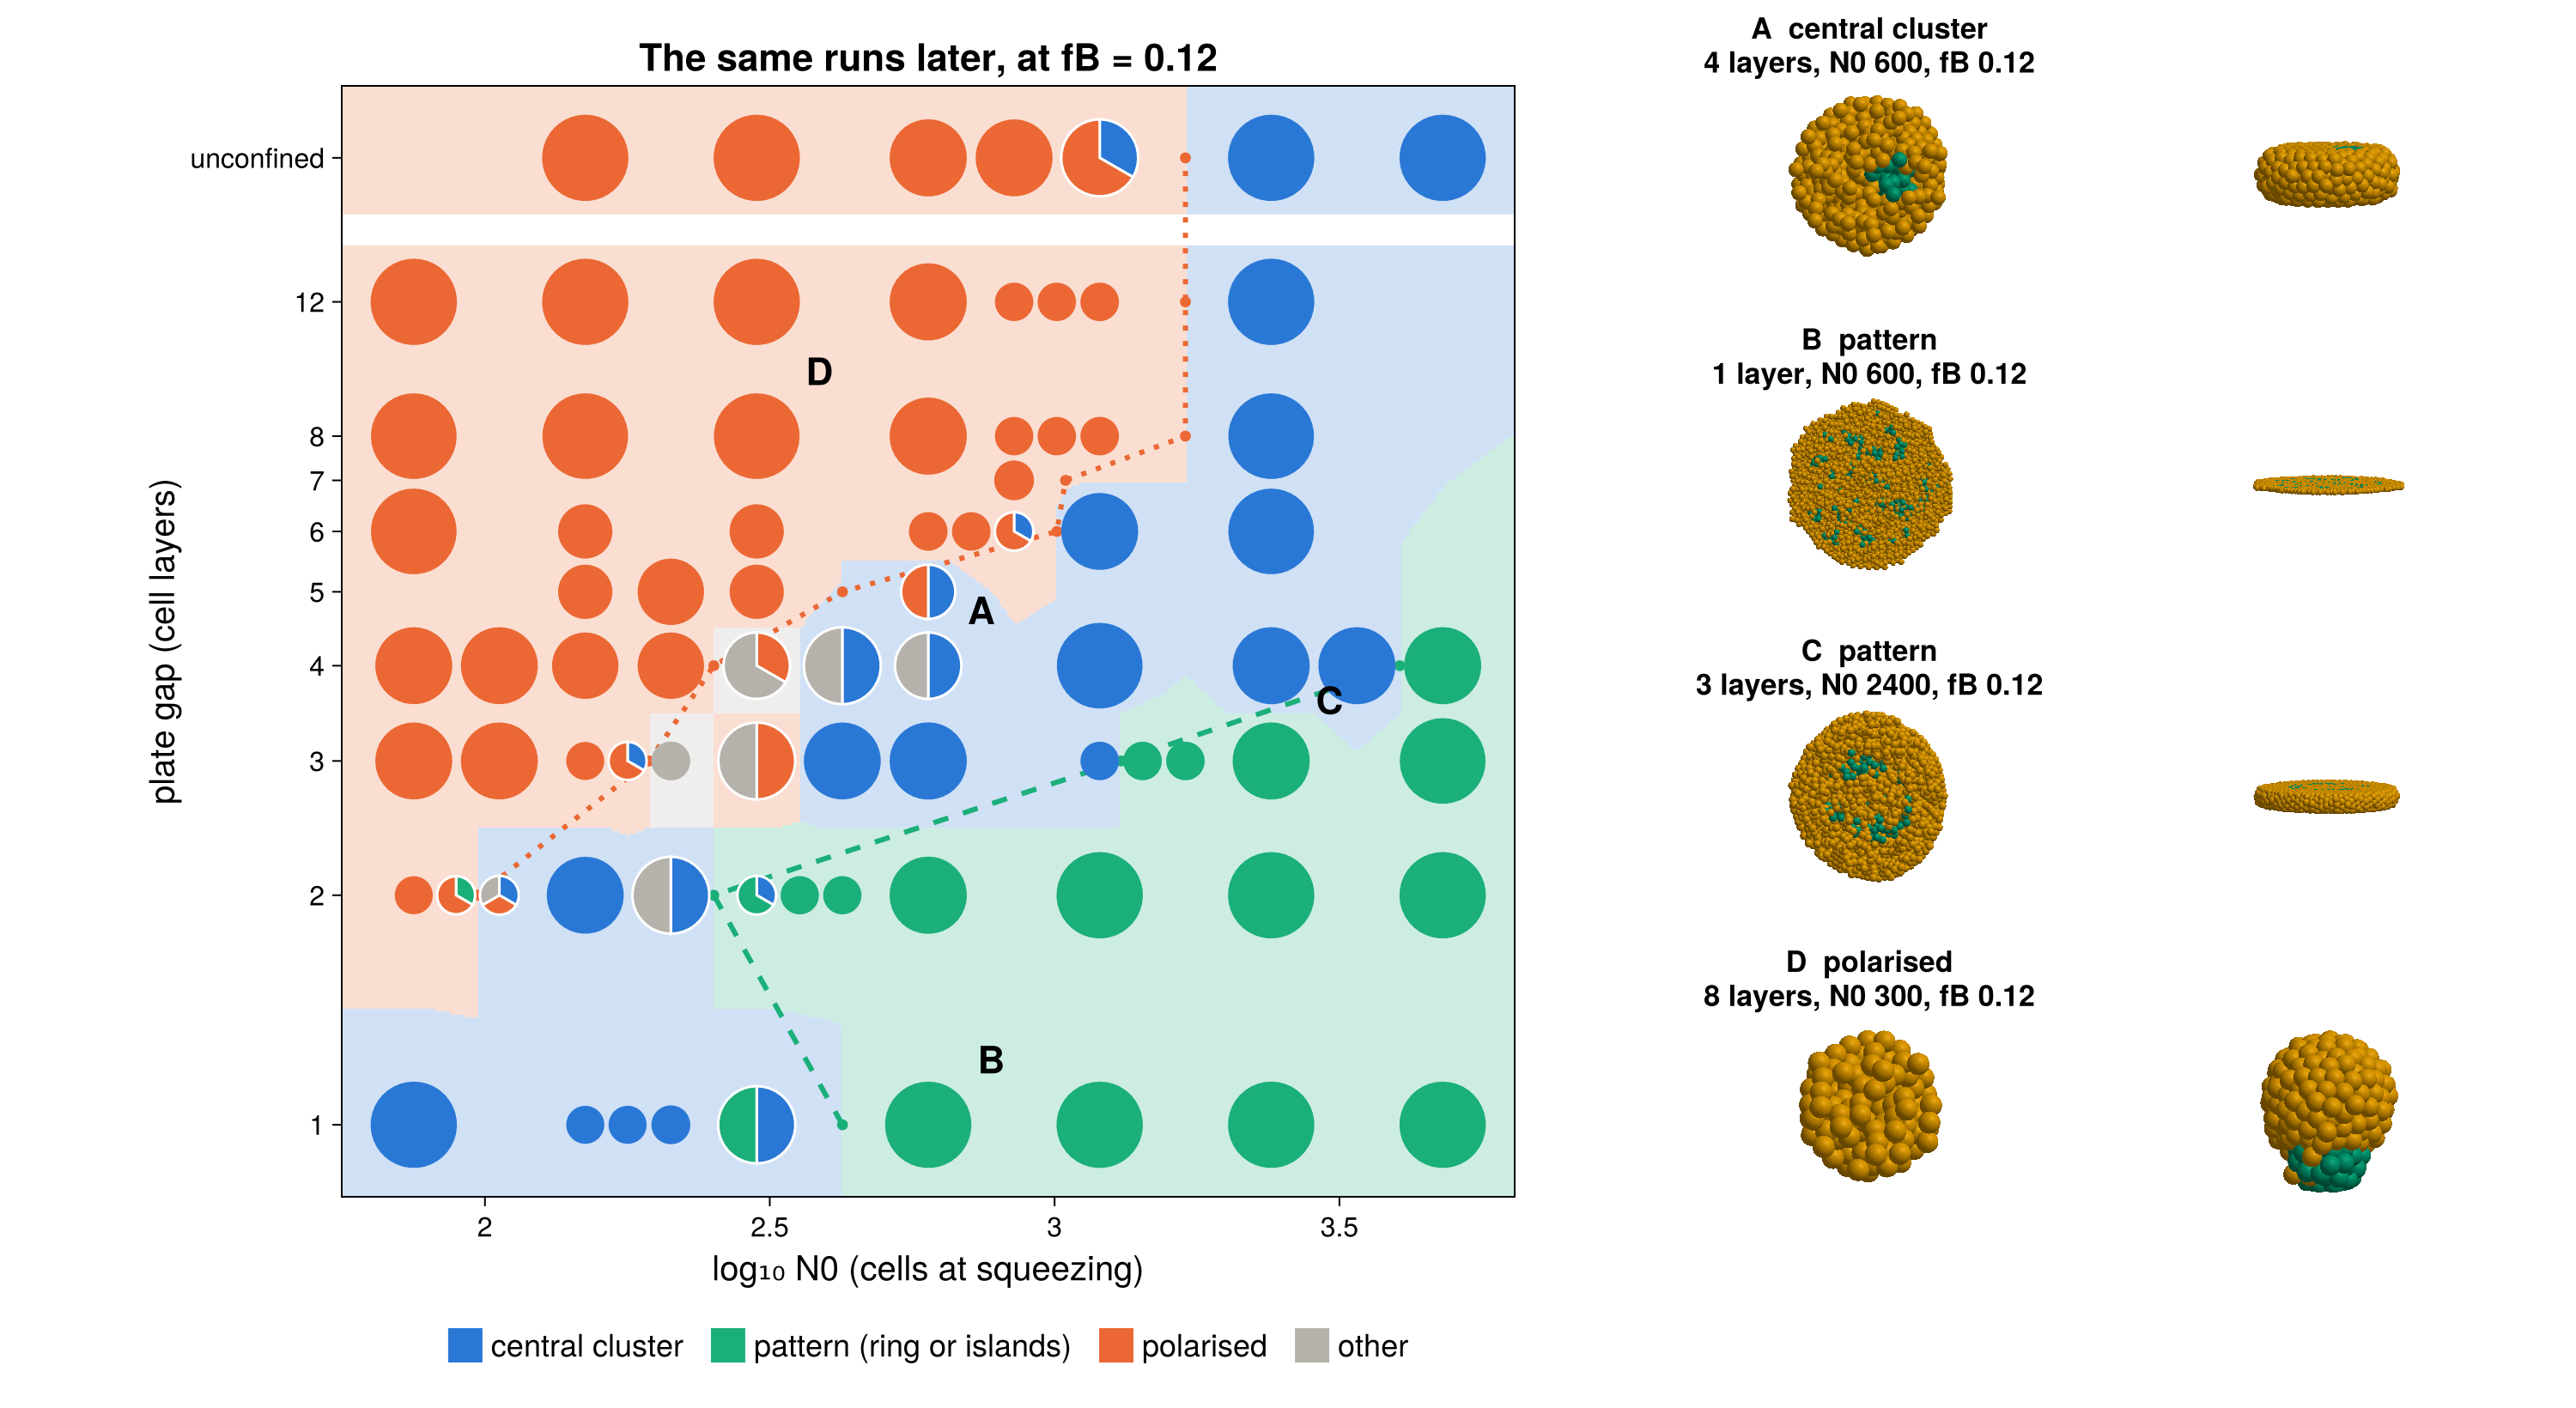
\includegraphics[width=\linewidth]{figures/phase_space_late.png}
    \caption{The same simulations, read when $12\%$ of the cells are $B$.}
    \label{phase-space-late}
\end{figure}


\section{Open points and possible improvements}

\begin{enumerate}
    \item Large aggregates that are not confined (or confined with a wide gap) neither pattern nor polarise before $B$ runs out. A free $B$ core can always round up, so it does not break into islands.
    \item The transition from a central cluster to a ring is gradual: near the threshold the cluster becomes loose and starts opening. Where we put the cut moves the thresholds by about one step in $N_0$.
    \item The value $\mu_{BB}=1.9$ is close to the point where $B$ dissolves into $C$ ($\mu_{BB}=1.85$).
    \item More simulations per point would sharpen the boundaries; the phase space has 2 or 3 per point, and 1 at $N_0=4800$.
\end{enumerate}



\newpage
\section{Parameters}

Table~\ref{parameters} gives the parameters of the July report (old) and the ones used now (new). Values in \chg{red} have changed. Entries of the $A$ state are shown as $\unused$, since $A$ cells no longer exist; in the matrices the order is $A, B, C$.

{\small                                 % smaller font size for the table
\begin{xltabular}{\textwidth}{
    >{\centering\arraybackslash}p{0.10\textwidth}   % symbol
    X                                               % description
    >{\centering\arraybackslash}p{0.21\textwidth}   % old value
    >{\centering\arraybackslash}p{0.21\textwidth}   % new value
}
\caption{Parameters of the July report (old) and of this report (new). Values in \chg{red} have changed.}
\label{parameters}\\
\hline
\textbf{Symbol} & {\textbf{Description}} & \textbf{Old (July)} & \textbf{New (October)} \\      % header
\hline
\endfirsthead
\hline
\textbf{Symbol} & {\textbf{Description}} & \textbf{Old (July)} & \textbf{New (October)} \\
\hline
\endhead
\hline
\endfoot
    $\Delta t$ & Timestep & 0.02 & \chg{0.015} \\
    $ r$ & Radius & 1 & 1 \\
     & Overlap factor & 0.3 & 0.3 \\
    $\alpha$ & Cell-ECM/cell-cell friction parameter & 0.9 & 0.9 \\
    $\tau_\text{div}^A$ & Average division time & 300 & \chg{-- (no $A$ cells)} \\
    $\tau_\text{div}^B$ & Average division time & 300 & 300 \\
    $\tau_\text{div}^C$ & Average division time & 750 & 750 \\
    $\sigma_\text{div}$ & Division time variability & 0.5 & 0.5 \\
    $\lambda$ & Global friction coefficient & 1 & 1 \\
    $\mu$ & Force range factor & $\begin{pmatrix}
        1.55 & 1.5 & 1.525 \\
        1.5  & 1.7 & 1.45 \\
        2.0  & 2.0 & 2.0
    \end{pmatrix}$ & $\begin{pmatrix}
        \unused & \unused & \unused \\
        \unused & \chg{1.9} & \chg{2} \\
        \unused & 2 & \chg{2.14}
    \end{pmatrix}$ \\
        & Neighbour range factor &  1 & 1 \\
    $F_{rep}$ & Repulsion force & $\begin{pmatrix}
        3 & 3 & 3 \\
          & 3 & 3 \\
          &   & 5.1
    \end{pmatrix}$ & $\begin{pmatrix}
        \unused & \unused & \unused \\
          & \chg{4.5} & 3 \\
          &   & \chg{6}
    \end{pmatrix}$ \\
    $F_{att}$ & Attraction force & $\begin{pmatrix}
        6 & 6 & 2.4 \\
          & 6 & 1.6 \\
          &   & 4.8
    \end{pmatrix}$ & $\begin{pmatrix}
        \unused & \unused & \unused \\
          & \chg{6.4} & 1.6 \\
          &   & \chg{3}
    \end{pmatrix}$ \\
    $p$ & Fixed transition rate from $A$ to $B$ & 0.009333 & \chg{-- (no $A$ cells)} \\
    $q$ & Fixed transition rate from $B$ to $C$ & 0.004667 & 0.004667 \\
    $K$ & Feedback parameter & 0.2 & \chg{-- (no feedback)} \\
    $\lambda_\text{wall}$ & Plate friction (cells closer than 0.05 to a plate) & -- & \chg{1.5} \\
     & Plates & -- & \chg{rigid} \\
    $L$ & Plate gap & -- & \chg{$2.1\,r \times$ layers} \\
    $\phi_B^0$ & Initial proportion of $B$ cells & -- & \chg{0.6 (central core)} \\
     & Readout: proportion of $B$ cells & -- & \chg{0.2} \\
    $n_i$ & Number of neighbours &  &  \\
    $n_i^X$ & Number of neighbours in state $X$ &  &  \\
    $\phi_X$ & Proportion of cells in state $X$ &  &  \\
    $T_0$ & Typical time scale & \SI{2}{\hour} & \SI{2}{\hour} \\
     & Time units per hour (from $q$) & -- & \chg{15} \\
    $R_0$ & Typical length scale & \SI{5}{\micro\meter} & \SI{5}{\micro\meter} \\
    $F_0$ & Typical force scale & \SI{20}{\pico\newton} & \SI{20}{\pico\newton} \\
\end{xltabular}
}

\textbf{Note on the old values.} They are the values in the table of the July report. The July simulations themselves used Sotiris' fusion set,
\begin{equation*}
    \mu = 2\begin{pmatrix} 1 & 0.91 & 1 \\ 0.91 & 1 & 1 \\ 1 & 1 & 1.07 \end{pmatrix}, \qquad
    F_\text{att} = 4\begin{pmatrix} 0.9 & 1 & 0.6 \\ 1 & 1.6 & 0.4 \\ 0.6 & 0.4 & 0.75 \end{pmatrix},
\end{equation*}
with $F_\text{rep}^{BB} = 3$ and $F_\text{rep}^{CC} = 5.1$, and Hookean plates. Compared with those, the only changes are $F_\text{rep}^{BB}$ ($3 \to 4.5$), $F_\text{rep}^{CC}$ ($5.1 \to 6$), $\mu_{BB}$ ($2 \to 1.9$), the plates (rigid, with friction $\lambda_\text{wall} = 1.5$) and the removal of the $A$ state. The $BC$ entries ($\mu_{BC}=2$, $F_\text{att}^{BC}=1.6$, $F_\text{rep}^{BC}=3$) and $q$ are unchanged. The typical time scale $T_0 = 2$~h does not match the $15$ time units per hour implied by $q$; it is worth checking.

\printbibliography

\end{document}
